\documentclass[11pt,a4paper]{article}
\usepackage[utf8]{inputenc}
\usepackage{amsmath}
\usepackage{amsfonts}
\usepackage{xcolor}
\usepackage{array}
\usepackage{amssymb}
%\usepackage{colortbl}
\usepackage{listings}
\usepackage{hyperref}
\usepackage{graphicx}
\usepackage[dutch]{babel}

\newcommand{\boxgreen}{\colorbox{green}{\color{black}Afgewerkt}}
\newcommand{\boxyellow}{\colorbox{yellow}{\color{black}Aan bezig}}
\newcommand{\boxred}{\colorbox{red}{\color{black}Onafgewerkt}}

\newcommand{\pack}[1]{$>$ #1.java \newline}

% Counter for the requirements
\newcounter{reqc} 
\newcommand{\reqID} {%
   \stepcounter{reqc}%
   \thereqc}

% Counter for the figures/images
\newcounter{figc}
\newcommand{\increaseFigID} {%
   \stepcounter{figc}%
   \thefigc}
   
% Command for setting text under table
\newcommand{\figID}[1]{\small \textit{Afbeelding \increaseFigID : #1} \\ \normalsize}

% Counter for the tables
   \newcounter{tabc}
\newcommand{\increaseTabID} {%
   \stepcounter{tabc}%
   \thetabc}

% Command for setting text under table
\newcommand{\tabID}[1]{\small \textit{Tabel \increaseTabID : #1} \\ \normalsize}


\author{David Sverdlov \\ dsverdlo@vub.ac.be \\ 3e Bachelor Computerwetenschappen}
\title{Bachelorproef AMuRate: Eindverslag }
\begin{document}
% Begin title page
\begin{flushleft}
\noindent 
\includegraphics[width=0.6\linewidth]{Pictures/vub_logo.jpg} 
\end{flushleft}
{\let\newpage\relax\maketitle} % don't let it set newpage

\begin{center}

\includegraphics[width=4cm]{Pictures/amr_gold_thick.png} 
\end{center}



\newpage
\tableofcontents

\newpage
\section{Inleiding} 
\label{sec:Inleiding}

	\subsection{Doel} 
	\label{sec:Doel}
Een bachelorproject is een belangrijke afsluiter van een bacheloropleiding. Dit project is volledig individueel en een vereiste tot het behalen van een bachelor diploma in de richting Computerwetenschappen aan de VUB. De uitdaging van dit bachelorproject is om een applicatie te ontwikkelen voor het mobiele platform Android. De applicatie moet gebruikers in staat stellen om muzieknummers op te zoeken en deze beoordelingen te kunnen geven. Die scores worden dan opgestuurd naar een grote database, waar later recommendeer algoritmen op zullen werken. Op die manier kunnen we nieuwe muziek aan de mensen voorstellen. De implementatie van die algoritmen valt niet binnen de scope van dit project. De promotor van dit project is Dr. Peter Vrancx en het project werd geassisteerd door Maarten Devillé.

	\subsection{Projectbeschrijving}
	\label{sec:Projectbeschrijving}
Hier gaan we het gebruik van de applicatie in dieper detail bespreken. Voor een visuele voorstelling refereer ik door naar sectie \ref{sec:GUIpics}: GUI.
\\
Gebruikers moeten eerst en vooral muziek kunnen opzoeken. Hier zal het hoofdscherm voor zorgen, waar men de zoekgegevens kan invullen. Er is een veld voor de titel van een lied in te vullen, en een veld voor de artiest- of groepsnaam. Beide velden hoeven niet tegelijk ingevuld te zijn, het volstaat dat er maar één veld ingevuld is. Wanneer een gebruiker op de zoekknop duwt zonder enige gegevens ingevuld te hebben, zal hij/zij een melding krijgen dat er eerst een zoekterm opgegeven moet worden.
\\ 

Een hulpknop informeert de gebruiker over het correct gebruik van de applicatie. Dit gebeurt door een pop up en kan gesloten worden door op OK te klikken. 
\\ 
 
Wanneer er geen werkende data connectie is, zij dat de data-connectie niet aan staat, of dat er geen beschikbaar netwerk in de buurt is, zal de gebruiker een melding krijgen dat hij een werkende data verbinding nodig heeft eer informatie gedownload kan worden. 
\\ 
	
Wanneer een gebruiker beschikt over een actieve data verbinding en minstens één zoekterm ingevuld heeft, zal de applicatie een verbinding maken met een grote externe database met muziekgegevens. De  database waar we gegevens van halen in dit project is die van Last.fm. Op het scherm zal een indicator tevoorschijn komen dat er een oproep behandeld wordt. Eens aangekomen, zal de Last.fm API de oproep behandelen en een antwoord vormen dat de opgevraagde informatie bevat. Eens dat antwoord door de applicatie ontvangen is, zal het resultaat aan de gebruiker getoond worden.
\\ 
	
Wanneer men kiest om de resultaten te bekijken, wordt er een lijst getoond met alle opties. Door op een van de resultaten te klikken, kan er naar het volgende scherm gegaan worden. Dat volgende scherm bevat meer informatie dan de beknopte optie waarop geklikt werd. 
\\ 
	
De gebruiker kan liedjes zoeken door het titelveld in te vullen, maar ook artiesten/groepen opzoeken door enkel iets in het artiestveld te schrijven. Wanneer de gebruiker enkel op artiest zoekt, gaan de gevonden resultaten doorverwijzen naar een gedetailleerde artiestenpagina. Op dat scherm is een kleine biografie te lezen van de artiest, een link naar een wiki-pagina, een afbeelding en een lijst van de top liedjes en top albums van die artiest. De gebruiker kan scrollen in beide lijsten en op elk item klikken om naar de respectievelijke gedetailleerde pagina's te gaan.
\\

Het gedetailleerde scherm van een lied geeft meer informatie over het lied in kwestie, zoals de duratie, albumnaam, artiestnaam, een afbeelding van het album\footnote{Indien er een afbeeldings URL beschikbaar is, anders een standaard blanco afbeelding.}. Indien er meer album informatie beschikbaar is, zal er een knop zijn waar gebruikers op kunnen klikken om naar de gedetailleerde pagina voor een album te gaan. 
\\ 	

Op het track scherm is er een deel van de pagina voorzien voor het scoresysteem. Naast de mogelijkheid om zelf eenmalig een score te geven (tussen 0 en 5 in sprongen van een halve ster), wordt ook de gemiddelde score weergegeven van alle scores voor dat lied (en het aantal scores waar het gemiddelde van berekend werd). Een boodschap informeert de gebruiker of hij al een score heeft gegeven voor dat lied, en wat die score was. Als er geen verbinding gemaakt kan worden met de server, zal de gebruiker hier ook een melding over krijgen. 
\\ 
	
Het gedetailleerde scherm voor een album toont informatie over het album en alle liedjes ervan. De gebruiker kan op elk lied klikken om naar het scherm te navigeren met meer informatie om een score te geven. Met een X-knop kan er terug gegaan worden naar het hoofdmenu.
\\ 
	
Wanneer een score toegediend wordt en er een werkende data verbinding is, moet de score niet alleen in de lokale database toegevoegd worden, maar ook naar de server gestuurd worden. In de externe database worden de scores opgeslagen samen met het tijdstip van het geven van de score, de id van het liedje, de titel, de artiest en de gebruiker die de score geeft. De gebruiker slagen we op via het unieke Android device nummer van het GSM toestel. Een gebruiker mag maar één score hebben per liedje in de databank.
\\

Vanaf het beginscherm kan de gebruiker ook op de knop `History' klikken om zijn geschiedenis te bekijken. Op het geschiedenis scherm zijn er vanboven 3 tabs te zien: `Search', `Tracks' en `Ratings'.  De tabs staan in een horizontale scrollview (er kunnen dus makkelijk bijgezet worden). De geschiedenis wordt dus onderverdeeld in zoekgeschiedenis (opgegeven zoektermen), trackgeschiedenis (bekeken tracks) en ratinggeschiedenis die alle gegevens scores bijhoudt. Elke onderverdeling heeft de optie om zijn geschiedenis te wissen.
\\

De gebruiker kan in elk scherm kiezen om op de menu-toets te duwen van zijn gsm, indien er een is. Dit opent het menu met enkele opties. Als de gebruiker op de optie `Refresh' klikt, zal de huidige pagina herladen worden. Dit kan handig zijn wanneer niet alle afbeeldingen geladen konden worden. De menu optie `Quit' zal de applicatie afsluiten. De menu optie `Change Language' zal een pop up tonen met de mogelijke talen waar de gebruiker uit kan kiezen. De laatste optie is `Set IP/port'. Hier kan de gebruiker wijzigen welke poortnummer gebruikt moet worden, of welk ip-adres.
	
	
	\subsection{Afkortingen en definities}
	\label{sec:Afkortingen en definities}
		\subsubsection{API}
		\label{sec:API}
		API staat voor Application Programming Interface en zorgt voor de communicatie tussen programma's, door de scheiding te vormen tussen verschillende lagen van abstracties.
		\subsubsection{XML/JSON}
		\label{sec:XML/JSON}
		XML of Extensible Markup Language is een van de meest gebruikte opmaaktalen die gestructureerde gegevens kunnen omzetten in platte tekst. Zo kan het makkelijk doorgestuurd worden.
		\newline
		JSON is aan afkorting van JavaScript Object Notation en is een alternatieve simpele manier om objecten voor te stellen als platte tekst.
		\subsubsection{HTTP}
		\label{sec:HTTP}
		HyperText Transfer Protocol is het medium tussen een webbrowser en een webserver. Die communicatie gebeurt door middel van URLs, die verwijzen naar `iets' op een webserver.
		\subsubsection{GUI}
		\label{sec:GUI}
		GUI staat voor Graphical User Interface en is een visuele vormgeving van een programma, dat door middel van knoppen, afbeeldingen, ... gebruikers toelaat om op een gebruiksvriendelijkere manier met de applicatie om te gaan.
		
		\subsubsection{MBID}
		\label{sec:MBID}
		De MBID van een liedje of artiest staat voor MusicBrainz Identifier. MusicBrainz is een grootschalige onderneming die een universeel, uniek muziek identificerings systeem implementeert. Een ID bestaat uit 36 karakters en kan gebruikt worden voor liedjes, artiesten, albums,...
	
		\subsubsection{REST}
		\label{sec:REST}
		REST staat voor Representational State Transfer en is een type van architectuur voor gedistribueerde systemen (zoals het World Wide Web), waarin een duidelijke onderscheiding wordt gemaakt tussen client en server. Clients kunnen oproepen doen naar de server, die de oproepen analyseert, een antwoord formuleert, en dat antwoord terug naar de client stuurt. De standaard sleutelwoorden voor oproepen in een RESTful architectuur zijn GET, POST, PUT en DELETE. Deze dienen respectievelijk om data te kunnen verkrijgen, aanmaken, wijzigen of opsturen.
		
		\subsubsection{JDBC}
		JDBC (Java Database Connectivity) is een API van Oracle die abstractie brengt in het verbinden met en beheren van databases. De API maakt het ook eenvoudig om informatie uit databases te filteren en de resultaten te gebruiken voor eender welke doeleinden.

\newpage		
\section{Achtergrond}
\label{sec:Achtergrond}
	\subsection{Last.fm API}
	\label{sec:Last.fm API}
Om informatie (over muziek in dit geval) te kunnen opzoeken, moet er gebruik gemaakt worden van een online database met een openbare API. \textit{Last.fm} is een muziek recommendation service met een enorme online muziek database, die geregistreerde gebruikers een gratis API aanbiedt. Zo mogen programmeurs mobiele/desktop programma's of web services bouwen, die beroep doen op hun data. De werking en gebruik hiervan wordt in detail besproken in sectie \ref{sec:Tracks omzetten}.

	
	\subsection{Codebeheer}
	\label{sec:Codebeheer}
		Voor dit project werd er gebruik gemaakt van Git als versiebeheersysteem, omdat het een gratis, eenvoudige en betrouwbare manier is om de broncode te beheren. Om updates in het project naar de repository te sturen wordt er gebruikt gemaakt van Github voor Windows. Nog een voordeel van deze dienst is dat Github de mogelijkheid biedt om snel en simpel websites te maken voor de bestaande projecten. Zo werd er een kleine website voor dit project opgesteld, die terug te vinden is op: \url{http://dsverdlo.github.com/AMuRate/}. Hier kan men de open-source broncode bekijken, het logboek of dit document raadplegen en de applicatie (.apk) downloaden voor Android 4.0+ toestellen. (Zie sectie \ref{sec:Installatie}:Installatie voor meer informatie over het installeren)
		
	\subsection{Naam en logo}
	\label{sec:Naam en logo}
		De naam van een project geeft meestal een kleine beschrijving van wat de applicatie doet/waar hij voor dient. AMuRate komt van `Android Music Rating'. Omdat het project vooral geïmplementeerd zou worden via een Android emulator en simpelweg `AMR' te kort en onduidelijk zou zijn, werd er gekozen voor AMuRate. Het logo (zoals te zien op de voorpagina) is een compositie van een 5-ster in een bol die iets weg heeft van een `dragonball' (uit de Japanse animatieserie DragonBall Z). In DBZ bestaan er maar 7 bollen op de hele wereld en wanneer die allemaal verzameld zijn, mag de beheerder een wens doen. Een beetje gelijkaardig aan hoe elke artiest hoopt 5 sterren (/ 7 dragon balls) te verzamelen. 
	In de ster zelf zijn drie gekleurde letters (AMR) te onderscheiden, naar de naam van de applicatie.
	
	
\newpage % hack for layout	
\section{Vereisten}
\label{sec:Vereisten}
Hieronder volgt een tabel die alle vereisten opsomt, met hun geïmplementeerde status. Deze tabel werd in de loop van het project meermaals bijgewerkt met verschillende statuskleuren, naargelang de level van afwerking per vereiste. Momenteel zijn ze allemaal groen omdat elke onderstaande functionaliteit geïmplementeerd is. \\

	% Get a nice table with colors running here, bro
	\hspace{-2em} \begin{tabular}{| l | l | c | r |}
	\hline
	ID 		& 	Categorie	&	Beschrijving						& Status 		\\ \hline \hline
	\reqID	&	Client		&	Titel en artiest kunnen invullen	& \boxgreen 	\\ \hline
	\reqID 	&	Client		&	Enkel op titel zoeken				& \boxgreen		\\ \hline
	\reqID	& 	Client		&	Enkel op artiest opzoeken 			& \boxgreen		\\ \hline
	\reqID 	& 	Client		&	Gedetailleerd lied weergeven		& \boxgreen 	\\ \hline
	\reqID 	& 	Client		&	Gedetailleerd artiest weergeven		& \boxgreen 	\\ \hline
	\reqID 	& 	Client		&	Gedetailleerd album weergeven		& \boxgreen 	\\ \hline
	\reqID	& 	Client		&	Scores beheren in lokale database	& \boxgreen  	\\ \hline
	\reqID	& 	Client		&	Geschiedenis beheren in database	& \boxgreen  	\\ \hline
	\reqID	& 	Client		&	Geschiedenis weergeven op scherm	& \boxgreen  	\\ \hline
	\reqID	& 	Client		&	Scores opsturen naar externe db		& \boxgreen		\\ \hline
	\reqID	& 	Server		&	Scores ontvangen op externe db		& \boxgreen		\\ \hline
	\reqID	&	Server		&	Scores ophalen uit externe db		& \boxgreen		\\ \hline
	\reqID	& 	Server		& 	Met meerdere klanten tegelijk verbinden	& \boxgreen		\\ \hline
	\reqID	& 	Beide		& 	Ongesyncte scores naar ext. db		& \boxgreen		\\ \hline
	\reqID	&	Beide		&	Kijk na of gebruiker al een score heeft gegeven	& \boxgreen		\\ \hline
	
%	\reqID	& 	necessity	&			& \boxred 		\\ \hline
%	\reqID	&	optional	&	Stream$/$preview 30sec songs		& \boxyellow 	\\ \hline
%	\reqID	&	optional	&	Caching implementeren				& \boxred 		\\ \hline
%	\reqID 	& 	optional	&	Onderzoek uitbreidbaarheid (ios?)	& \boxred 		\\ \hline
%	\reqID 	&	optional	&	Informatie ophalen van media speler & \boxred 		\\ \hline
	%\hline	
	\end{tabular} \\ \newline
	\tabID{Vereisten van het project met uitleg en implementatiestatus.} 
	
	Zoals in de projectbeschrijving reeds gezegd werd, bestaat het project uit twee afzonderlijke delen, die verbonden kunnen worden door een internetverbinding. Aan de client-kant is er de applicatie op Android, en aan de server-kant een data-collection server die scores verzameld en geregeld gebruikt wordt voor recommendeer algoritmen. De server-kant is een kleiner pakket dan de client-kant, maar niet minder belangrijk. 
	\\ \newline



\newpage % hack for layout	
	%%%%%%%%%%%%%%%%%
	% Implementatie %
	%%%%%%%%%%%%%%%%%
\section{Implementatie}
\label{sec:Implementatie}

	\subsection{Android applicatie}
	\label{sec:Android applicatie}	
		\normalsize  
		De broncode van het project is opgedeeld in 3 packages: \textit{gui, objects en services}. Hier een overzicht van de packages en hun inhoud:\\
		
		 \textbf{com.dsverdlo.AMuRate.gui} \newline		
		 \pack{AlbumActivity}
		 \pack{AnimationView}
		 \pack{ArtistActivity}
		 \pack{BlankActivity}
		 \pack{HistoryActivity}
		 \pack{MainActivity}
		 \pack{SearchArtistActivity}
		 \pack{SearchResultsActivity} 
		 \pack{TrackActivity}
		 
		\textbf{com.dsverdlo.AMuRate.objects} \newline
		\pack{Album}
		\pack{AMuRate}
		\pack{Artist}
		\pack{History}
		\pack{Rating}
		\pack{Track}
		
		\textbf{com.dsverdlo.AMuRate.services} \newline
		\pack{DatabaseSyncer}
		\pack{DownloadImageTask}
		\pack{DownloadLastFM}
		\pack{InternalDatabaseHistoryAdapter}
		\pack{InternalDatabaseManager}
		\pack{InternalDatabaseRatingAdapter}
		\pack{ServerConnect}
		\pack{ServerConnectMySQL}
		\pack{ServerConnectPHP}
		
		 In het \textit{GUI} package zitten alle activities\footnote{Dit is de naam van een scherm in Android} en alle klassen die te maken hebben met het uiterlijk van de applicatie. Elk scherm om iets op weer te geven heeft een eigen activity nodig. \\
		 
		In het \textit{objects} package zitten de objecten/units/simpele java klassen, die abstractie brengen in het project. Het is ook hier dat de globale applicatie `AMuRate.java' zit.  \\
		
		Package \textit{services} bevat de klassen die instaan voor verschillende diensten die moeten gebeuren in de applicatie. De DownloadLastFM klasse doet de oproepen en download antwoorden van de Last.fm API, en de DownloadImageTask haalt alle afbeeldingen per HTTP binnen. De InternalDatabaseManager klasse is ook een dienst die verleend wordt, namelijk het beheren van de interne database. Per tabel in de interne database is er een adapter klasse die alle SQL bevat. De ServerConnection klasse staat in voor de verbinding met de externe database. Momenteel zijn er twee mogelijke verbindingen geimplementeerd. Die worden in detail besproken in sectie \ref{sec:Netwerkverbinding}.

	\subsection{Java server}
	\label{sec:Java server}
	De server code bestaat uit drie bestanden in één package. De `Server.java' is het bestand dat eenmalig opgestart moet worden om de server te doen draaien. De server draait standaard op poort 2005. Een ander poortnummer kan meegegeven worden door de server in commandline op te starten en een nieuw poortnummer mee te geven. \\
	Wanneer een client probeert te verbinden met de server, zal de server een aparte thread opstarten hiervoor. Op die manier kunnen er meerdere clients tegelijk hun informatie van de server krijgen zonder dat ze op elkaar moeten wachten. Zo'n thread zal een instantie van `ServerConnectionTask.java' zijn. Die task gaat dan aan de `ExternalDatabaseConnection.java' vragen om scores in- of uit de database te halen. Alle SQL is behouden in één klasse en afgeschermd van de rest. \\
	
	\textbf{com.dsverdlo.AMuRate.server} \newline
	\pack{ExternalDatabaseConnection}
	\pack{Server}
	\pack{ServerConnectionTask}
	
	\subsection{Data flow}
	\label{sec:Data flow}
	Om de overgangen tussen alle schermen overzichtelijk te illustreren, werd er een Data Flow Diagram gemaakt. Zie onderstaande afbeelding: \newline
	
	\hspace{-3em} 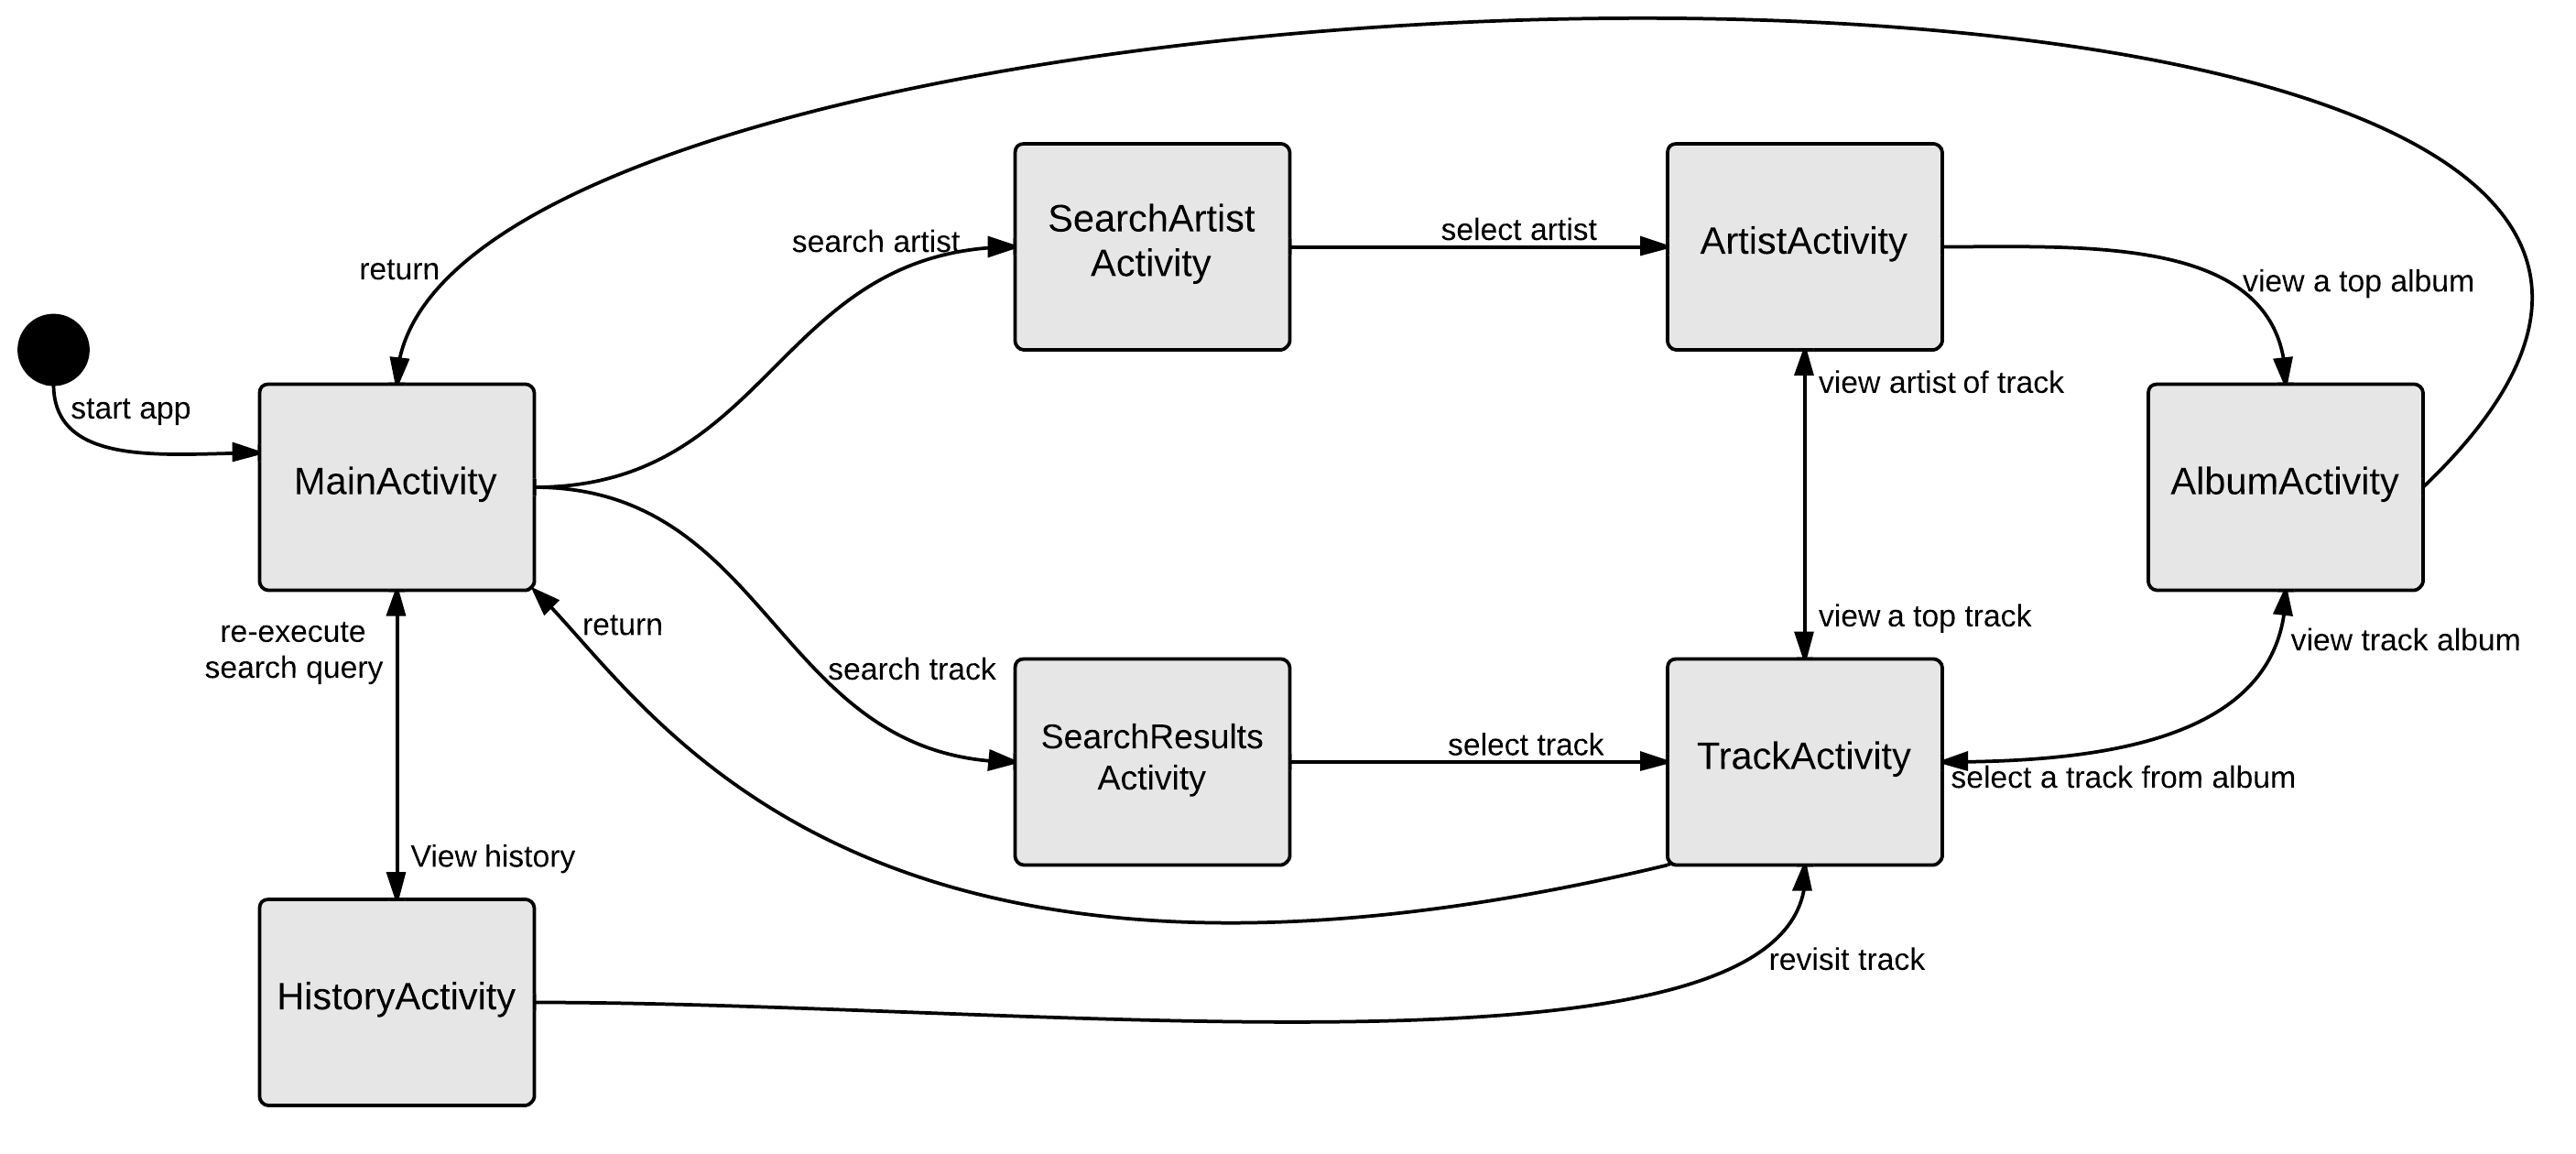
\includegraphics[scale=0.14]{Pictures/Dataflow4.png} \newline
	\figID{De data flow tussen alle activies.} 
	
	In het diagram zien we twee pijlen vertrekken vanuit MainActivity naar de SearchActivities. Wanneer enkel een artiest ingevuld werd, zal de applicatie naar de SearchArtistActivity gaan. Vanaf dat er ook een titel ingevuld wordt, gaat de applicatie naar SearchResultsActivity. Dit wordt nog besproken in hoofdstuk \ref{sec:Technisch}: Technisch  en is visueel te zien in hoofdstuk \ref{sec:GUIpics}: GUI.
	
	\subsection{Databases}
	\label{sec:Databases}
	Er zijn twee databases in dit project. Eén lokale, op elk toestel met een AMuRate applicatie, en één grote centrale database op een server. De lokale databases houden enkel data bij van hun gebruikers, terwijl de externe de scores van iedereen verzamelt. We zullen nu beide databases bespreken.
	
	\subsubsection{Lokale Database}
	\label{sec:Lokale Database}
	De lokale database moet data bijhouden die offline geraadpleegd zou willen worden. Hiermee bedoelen we onder andere geschiedenis van de ingevoerde zoekopdrachten, bekeken liedjes en de laatst gegeven scores. Aangezien deze applicatie vooral beroep doet op een actieve internetverbinding, zal er niet meer dan dat opgeslagen worden. \\ \newline 
	De lokale database bevat dus twee tabellen en de operaties op deze tabellen gebeuren d.m.v. adapters. Die adapters maken de brug tussen procedures als `read-X-from-database' en SQLite statements (zoals "SELECT X FROM tablename"). Er is dus één adapter per tabel. \newline
	 \\ \newline
	 \begin{itemize}
		\item Ratings table \newline
		
		\begin{tabular}{| l | l | l | }
		\hline
		 Naam		& Type		& Sleutel		\\
		 \hline 
		 id 		& integer 	& primary key 	\\
		 date 		& integer	& 				\\
		 rating 	& float 	& 				\\
		 mbid 		& text 		& 				\\
		 title 		& text 		& 				\\
		 artist 	& text 		& 				\\
		 sync		& integer 	& 				\\
		 \hline
		\end{tabular} \newline
		\tabID{Het model van de Rating tabel in de lokale database.}  

		De laatste kolom in de tabel is een `sync bit'. Dat betekent dat hij enkel de waarde 0 of 1 kan hebben. Wanneer hij waarde nul heeft, betekent het dat de score nog niet verzonden is naar de externe database. Dit kan voorvallen als er slechte verbinding is, of de server even uit zou staan bijvoorbeeld. Wanneer dat voorvalt, zal de functie die de score wou opsturen een negatieve response krijgen. Omdat we checken of de score goed is aangekomen, kunnen we detecteren wanneer het zou falen en kunnen we de score lokaal opslagen. De DatabaseSyncer zal de score opsturen eens er terug verbinding is en de sync bit op waarde 1 zetten, zodat we weten dat hij opgestuurd is. 
		
		\item Geschiedenis table \\
		
		\begin{tabular}{| l | l | l | }
		\hline
		Naam	& Type		& Sleutel		\\
		\hline
		id 		& integer 	& primary key 	\\
		key		& integer	&				\\
		date 	& integer 	& 				\\
		artist 	& text 		& 				\\
		title 	& text 		& 				\\
		mbid 	& text 		& 				\\
		\hline
		\end{tabular} \newline
		\tabID{De Geschiedenis tabel in de lokale database.} 
	
		Het `key' veld, in de tweede rij, is een lokale identificeerder die onderscheid gaat maken tussen een zoek-geschiedenis-record en een track-viewed-geschiedenis. Deze twee soorten records staan samen in één tabel omdat ze, op één veld na, alle velden gemeenschappelijk hebben. Bij track-viewed-geschiedenis gaan we de MBID mee opslagen om sneller de informatie terug te kunnen downloaden. Voor de zoek-geschiedenis-records is dit veld leeg in de database.
	 \end{itemize}
	
\newpage
	\subsubsection{Server Database}
	\label{sec:Server Database}
	\label{sec:Extdb}
	De externe database moet enkel scores van gebruikers verzamelen. Om verschillende gebruikers te onderscheiden zal er een user ID bijgehouden worden. Deze user ID zal het uniek Android ID zijn. De tabel zal er dan zo uitzien: \\ \newline
		\begin{tabular}{| l | l | l | }
		\hline
		 Naam		& Type		& Sleutel		\\
		 \hline 
		 idRatings 	& integer 	& primary key 	\\
		 MBID 		& text 		& 				\\
		 Artist		& text 		& 				\\
		 Title 		& text 		& 				\\
		 Rating		& float 	& 				\\
		 Date 		& integer 	& 				\\
		 User		& text 		& 				\\
		\hline
		\end{tabular}
		\label{tab:extDB}
	
	\tabID{De Rating tabel layout van de database op de server.} 
		
	De synchronisatie van deze tabel met de lokale ratings database gebeurt via een DatabaseSyncer klasse in de applicatie. Die klasse zal wanneer er ongesyncte scores in de lokale database opgeslagen staan, de scores naar de server sturen zodat ze terug gelijk lopen. Dit wordt verder in detail besproken in sectie \ref{sec:Database Syncing}: Syncing.
	
\newpage %hack for layout
%%%%%%%%%%%%%%%%%%%%%%%%%
%%	Technische details %%
%%%%%%%%%%%%%%%%%%%%%%%%%
\section{Technische beschrijving}
\label{sec:Technisch}

	\subsection{Netwerkverbinding}
	\label{sec:Netwerkverbinding}
	De AMuRate data collection server is een combinatie van een Java server en een MySQL database, die momenteel lokaal op mijn laptop draait. Deze database bevat één grote tabel, zoals in deze tabel:\ref{tab:extDB} te zien is. Wanneer een score gegeven zou worden op de applicatie, probeert de applicatie een socket\footnote{Standaard communicatiemiddel tussen programma's en computerprocessen} te openen op dezelfde poort als de server. Als de server draait, is er een serversocket die constant luistert naar nieuwe verbindingen. Als die serversocket een oproep van de applicatie opmerkt, zal die een nieuwe Thread aanmaken voor die verbinding vast te maken. De applicatie zet de score op de out-stream van zijn socket, waarna de serversocket de score van zijn in-stream afhaalt. De score is nu goed op de server aangekomen. \\
De server geeft de score dan mee aan zijn ExternalDatabaseConnection klasse, die de nodige SQL instructies zal opstellen om de score in de database te kunnen voegen. Om de SQL op te sturen, maken we gebruik van een JDBC. Dit is een Java API die het makkelijk maakt om Java programma's te verbinden met databases, data te query-en en resultaten van queries te behandelen. \\

	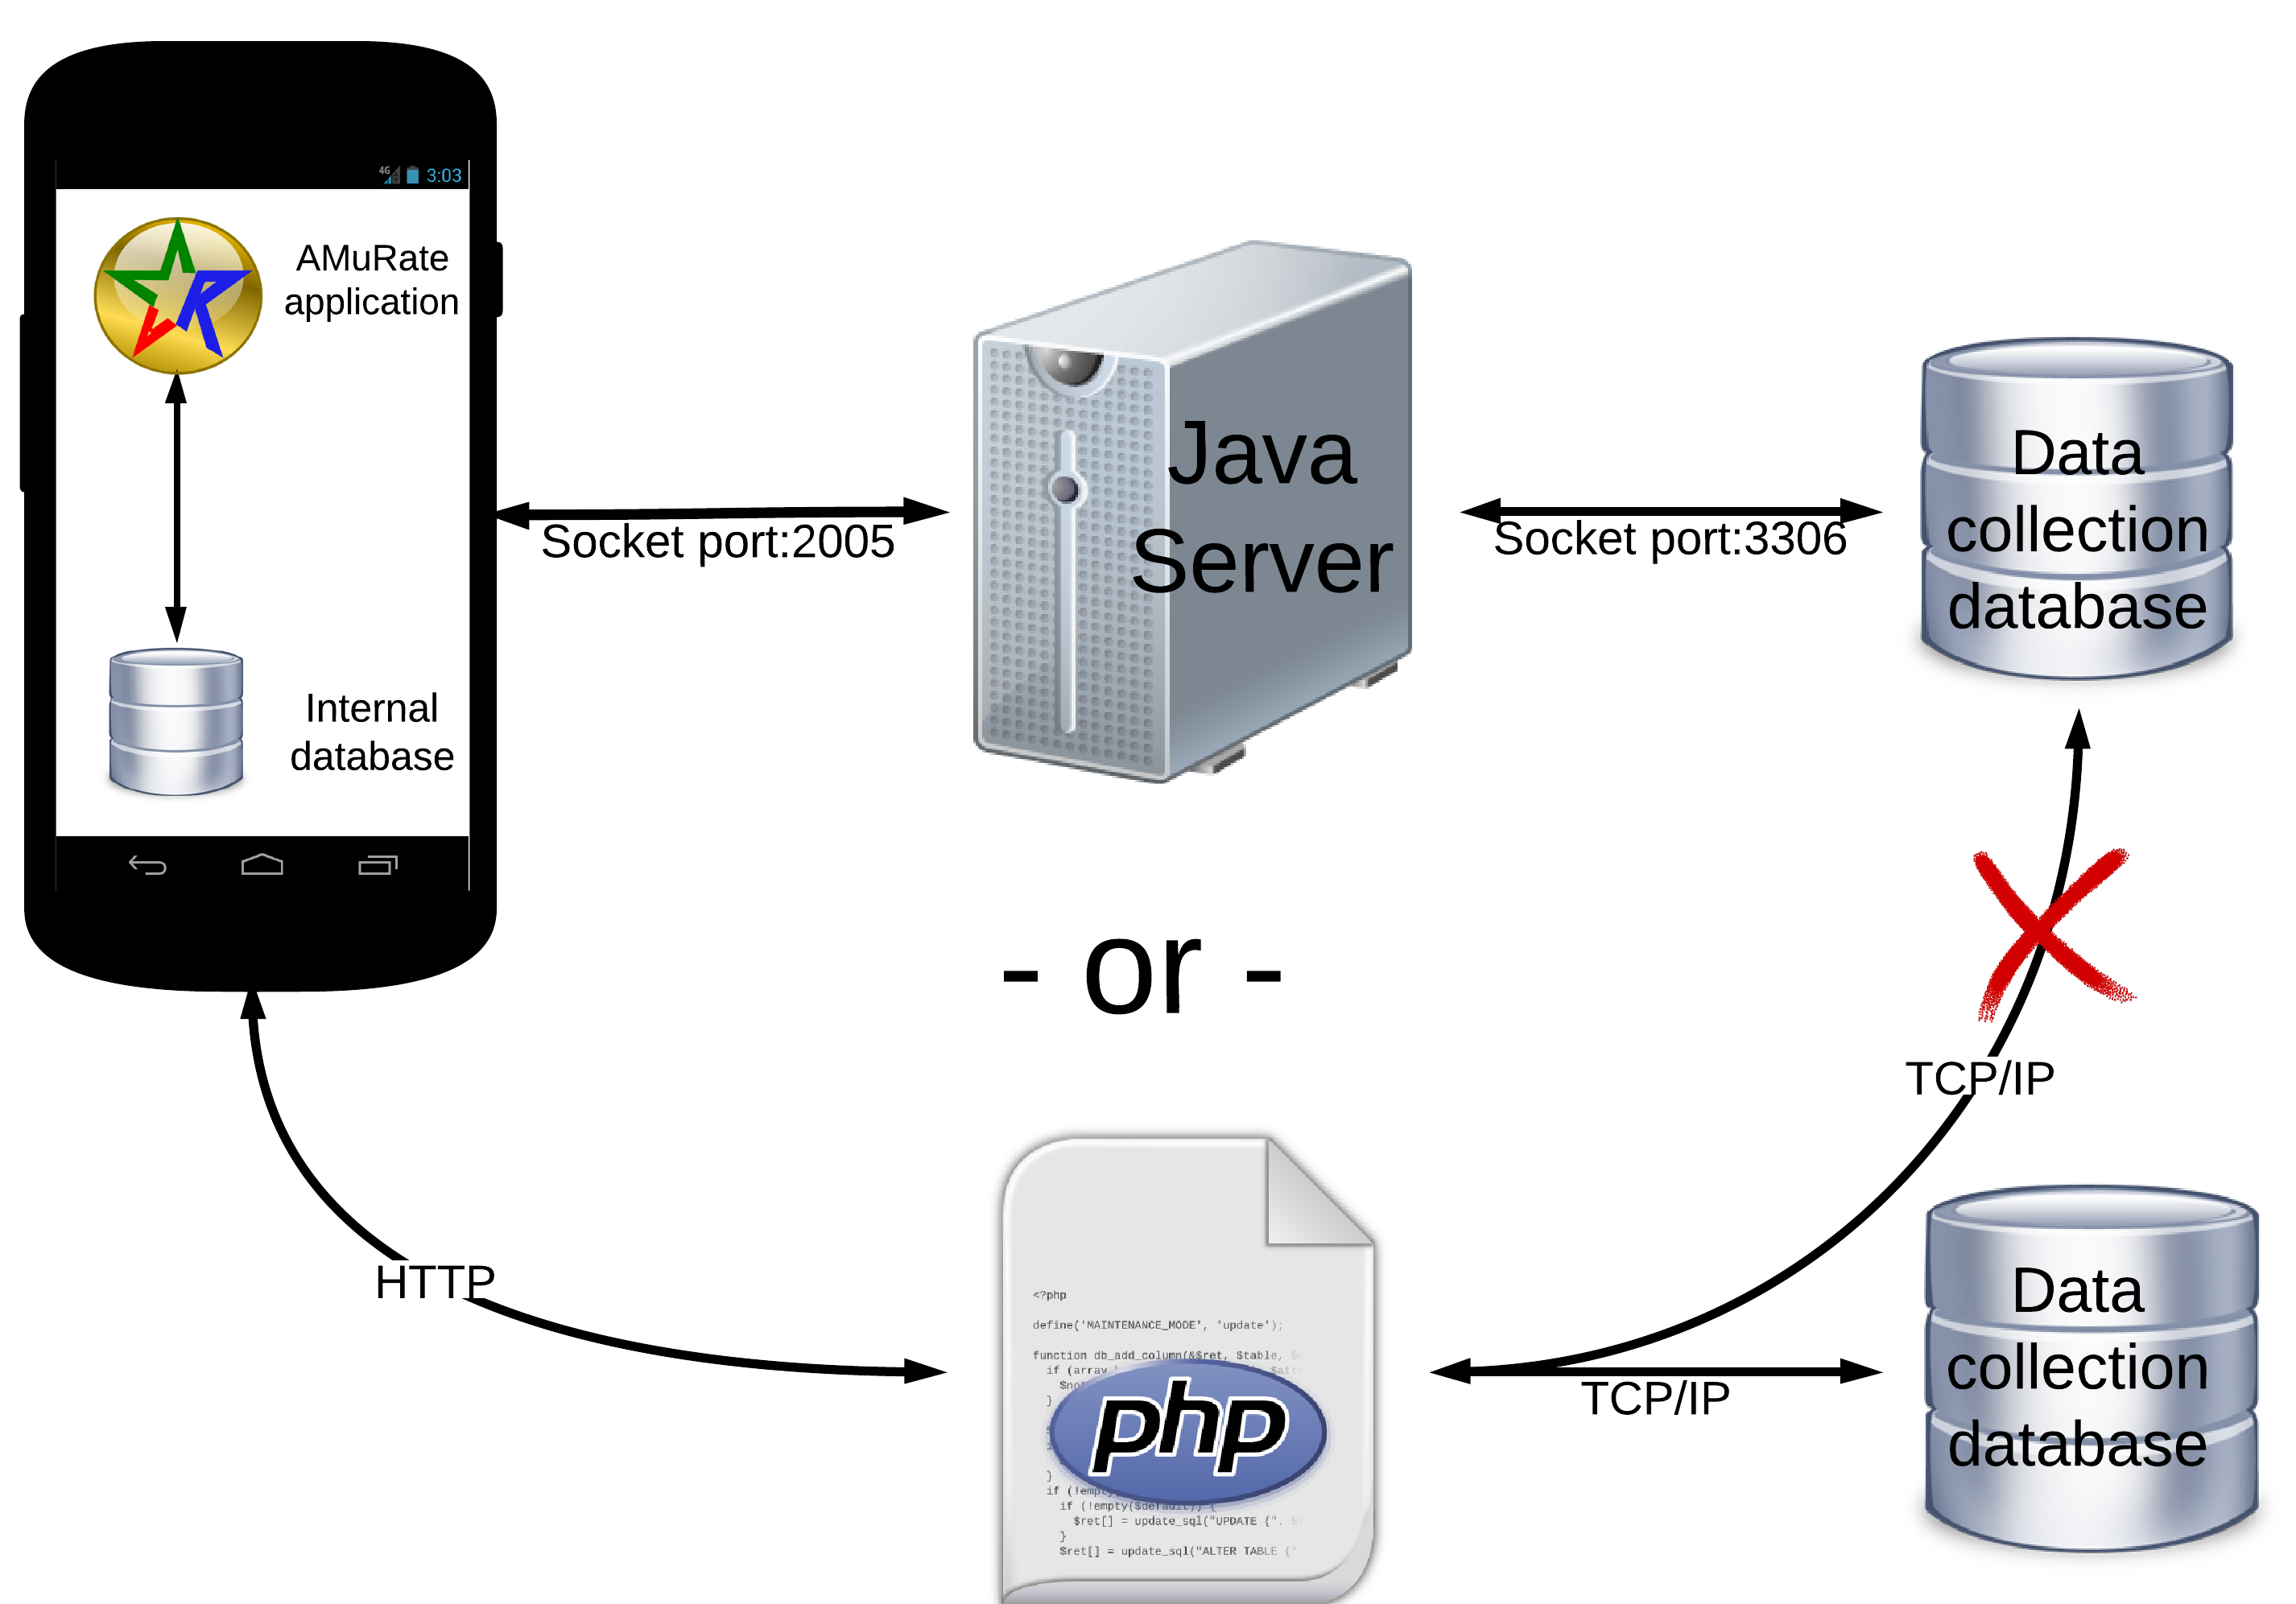
\includegraphics[scale=0.12]{Pictures/Sockets3.png} \newline
	\figID{Overzicht van de server verbindingen.}

	In de bovenstaande afbeelding zien we vanaf de telefoon ook een HTTP verbinding naar een PHP script vertrekken. Dit is een back up voor wanneer de server offline zou zijn. De bedoeling van de PHP scripts is dat ze ook scores kunnen sturen naar dezelfde MySQL database. Omdat die database momenteel lokaal op mijn computer draait, kunnen die PHP scripts er niet continue connectie mee maken. Daarom werd er een exacte kopie gemaakt van de database. Aangezien de bedoelde verbinding op dit moment niet doorloopt, werd er een rood kruis door gezet. Deze situatie met twee verschillende databases heeft enkel nut tijdens de test evalutie en zal verholpen worden wanneer de Java Server en MySQL database op een stabiele server draaien. De (op de afbeelding) onderste MySQL database wordt gehost op een gratis webhosting service. \\
	Om dit allemaal te implementeren, is er in de code van de applicatie een klasse ServerConnect, die de mogelijkheid heeft te kiezen welke service te gebruiken. Aangezien de Java Server en de MySQL database tijdens dit project lokaal op mijn laptop hebben gedraait, kon ik de app toch testen (en laten testen) op andere mobiele telefoons, netwerken en locaties d.m.v de PHP scripts. Dit is niet even veilig/zeker als een socketverbinding, maar we kunnen wel problemen met de overdracht opvangen en hiernaar handelen.


	\subsection{Uniek datamodel}
	\label{sec:Uniek datamodel}
	Gebruikers mogen maar één score per lied geven. Records in de database hebben dus `MBID' en `User' als primaire sleutel. Dit is deels om spam te voorkomen en deels om een eerlijk gemiddelde te kunnen maken van scores. Wanneer een lied wordt geladen in de applicatie, wordt er in de databases gekeken of de gebruiker al een score heeft gegeven voor de MBID geassociëerd met het gekozen lied. Wanneer de gebruiker al een score heeft gegeven, zal hij/zij geïnformeerd worden met de gegeven score. 
	Als er geen verbinding is met de externe database, kunnen we op die moment niet achterhalen of de gebruiker al eens een score heeft gegeven aan dat lied. We slagen de score dan even lokaal op tot er terug een verbinding op stand kan komen en updaten dan de gegeven score. Zie sectie\ref{sec:Database Syncing} Database Syncing.
	
	\subsection{Soorten zoekopdrachten}
	\label{sec:Verschillende zoekopdrachten}
	Op het hoofdscherm zijn er twee inputvelden; `artiest' en `titel'. Gebruikers kunnen kiezen welke velden ze wel en niet willen invullen om te vinden wat ze zoeken. Dat levert ons 4 opties;
		\begin{itemize}
			\item \textbf{Geen artiest en geen titel} \\
		Aangezien er niets is ingevuld, kan er ook niets opgezocht worden. De gebruiker krijgt een boodschap te zien dat er minstens één veld ingevuld moet zijn. \\
		
			\item \textbf{Wel artiest en geen titel} \\
		Wanneer enkel de artiestnaam (of groepsnaam) ingevuld wordt, zal er een zoekopdracht gedaan worden naar alle artiesten/groepen met een gelijkaardige naam als de querie. Als er resultaten gevonden zijn, kan de gebruiker kiezen uit een lijst van resultaten. Wanneer een resultaat met een afbeeldingsurl kwam, kunnen we er een afbeelding bij tonen om het selectieproces te vergemakkelijken. Wanneer de gebruiker op een van de opties klikt zal hij doorgewezen worden naar de ArtistActivity pagina van die artiest/groep. \\
		
			\item  \textbf{Geen artiest en wel titel} \\
		Er wordt gezocht naar alle liedjes met een gelijkaardige titel als die van de querie. De artiesten kunnen varieren en worden niet gefilterd. Als er resultaten gevonden worden, kan de gebruiker op eender welke klikken om naar de TrackActivity te gaan, waar hij/zij een score kan geven.\\
				
			\item  \textbf{Wel artiest en wel titel} \\
		Wanneer beide velden ingevuld worden wordt er dezelfde aanvraag als hier net boven gestuurd naar de Last.fm API, maar in de querie voegen we de artiestnaam toe. De filtering gebeurt op de Last.fm API zelf, en indien er matches zijn voor beide gegevens, kan de gebruiker erop klikken om naar TrackActivity te gaan.
		\end{itemize}
		
		
			\subsection{Last.fm}
	\label{sec:Tracks omzetten}
	
Om data uit de Last.fm database te halen moet er een call (oproep) gestuurd worden via HTTP. Deze gebeurt door een GET oproep naar de Last.fm server te sturen. Die server gaat op zijn beurt antwoorden met een XML object (of JSON op aanvraag). De architectuur van client$<->$server die hier gebruikt wordt heet `REST(ful)'. \\

De url van de aanvraag bestaat uit 3 delen; de basis van de API, de methode met zijn parameters en de api-key. De basis is altijd `ws.audioscrobbler.com/2.0/' en de methode is van de vorm `?method=category.function'. De parameters in de vorm van `\& param1=value1\& param2=value2'. Een api-key is een string van 32 karakters en gratis te verkrijgen door te registeren bij Last.fm.
De Last.fm API biedt tientallen methodes aan, zoals bijvoorbeeld artist.search, artist.getTopAlbums, artist.getTopTracks, track.getInfo, track.search, track.getTags, album.search, album.getBuyLinks, ... . \\
Voor een overzicht van alle methoden verwijzen we door naar hun website: \url{http://www.last.fm/api}. \\ 

De methoden die in dit project gebruikt worden zijn: \\

\hspace{-4em} \begin{tabular}{| l | l | l |}
\hline
	Activity 				&	Methoden			& Uitleg \\ \hline
	MainActivity			&	track.search 		& Gebruiker zoekt op title (en artiest) \\
	"						&	artist.search 		& Gebruiker heeft enkel artiest ingevuld \\ \hline
	SearchResultsActivity	&	track.getInfo		& Gebruiker klikt op een lied optie \\ \hline
	SearchArtistActivity	&	artist.getInfo		& Gebruiker klikt op een artiest optie \\ \hline
	TrackActivity			&	artist.getInfo		& Gebruiker wilt artiest van lied bekijken \\
	"						&	album.getInfo		& Gebruiker wilt album van lied bekijken \\ \hline
	ArtistActivity			&	track.getTopTracks	& Toont top liedjes van artiest \\
	"						&	album.getTopAlbums	& Toont top albums van artiest  \\ \hline
	AlbumActivity			&	track.getInfo		& Gebruiker wilt een lied v/h album zien \\ \hline
	HistoryActivity			&	track.getInfo		& Gebruiker wilt een lied herbekijken \\
\hline
\end{tabular}
	\tabID{Een overzicht van alle oproepen in de applicatie.} 

	Een tegengekomen probleem in dit project is het feit dat de Last.fm API oproepen (zoals track.getInfo en track.search) antwoorden met verschillende representaties. Om een voorbeeld te geven: hieronder bevinden zich de resultaten van twee oproepen met verschillende methoden voor het lied `Bohemian Rhapsody' van Queen. Er kan opgemerkt worden dat in het eerste resultaat `artist' een top level attribuut is van `track'. In het tweede snippet is `artist' een JSON object met zijn eigen velden. Om zo'n object\footnote{In dit document gebruiken XML notatie omdat deze makkelijker leesbaar is dan JSON, maar in de broncode wordt er enkel met JSON gewerkt.} om te zetten in een `Track' klasse, moet de Track klasse een onderscheid maken in wat voor soort object gebruikt wordt om de klasse te initialiseren. De beste oplossing hiervoor is om per representatie een loadFromX functie te maken die weet hoe X eruit ziet en waar alle informatie staat. Als we net een oproep hebben gedaan met methode `track.search', zullen we de Track.loadFromSearch oproepen. Voor een oproep met `track.getInfo', roepen we Track.loadFromInfo op. \\
	
	Track.search resultaat:\\
	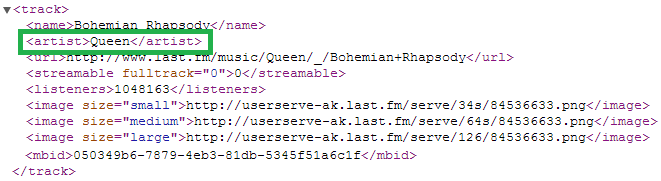
\includegraphics[scale=0.8]{Pictures/track_search2.png} \\ \newline
	\figID{Resultaat van track.search GET oproep voor Bohemian Rhapsody - Queen.}

	Track.getinfo resultaat: \\
	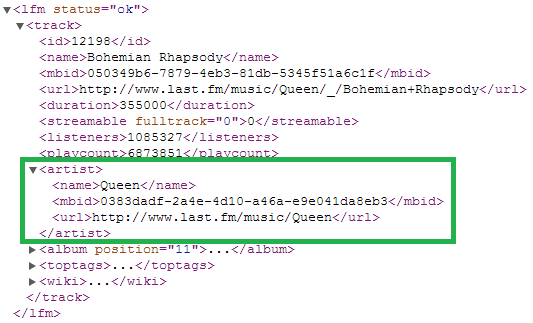
\includegraphics[scale=0.8]{Pictures/track_getinfo2.png}\\ \newline
	\figID{Resultaat van track.getInfo GET oproep voor Bohemian Rhapsody - Queen.}
	
	
	
	\subsection{Beveiliging}
	\label{sec:Beveiliging}
	De beide databases zijn beschermd tegen SQL-injecties door het het gebruik van preparedStatements, in plaats van String formattering. Wanneer er enkel validatie op de user input wordt gedaan, zou het nog mogelijk zijn dat de gebruiker een extra SQL-instructie meestuurt.
	Een preparedStatement compileert een SQL-instructie op voorhand en laat toe om erna nog parameters te binden. De preparedStatement heeft dan zijn executiepad volledig uitgewerkt, wat het onmogelijk maakt om een SQL-injectie in te voegen die, bijvoorbeeld, tabellen dropt. \\
	
	Om scores te posten via de PHP scripts, moet er een geheime applicatie code meegstuurd worden om te verifiëren dat de oproep wel van de AMuRate applicatie komt.
	
	
	\subsection{Database Syncing}
	\label{sec:Database Syncing}
	Het kan voorkomen dat de Java server of de MySQL database offline zijn voor een bepaalde onverwachte periode/reden. Als de gebruiker een score wilt geven en de applicatie vaststelt dat er geen verbinding tot stand kan komen, wordt de score tijdelijk opgeslagen in de lokale database. Hier komt de kolom `Sync' handig in voor, want we zetten die sync bit dan op 0 (=unsynced, 1=synced). Telkens wanneer de gebruiker verwisselt tussen schermen in de applicatie, zal de DatabaseSyncer kijken of er unsynced scores in de lokale database zitten. Dit gebeurt volledig op de achtergrond en is onzichtbaar voor de gebruiker. Wanneer er unsynced scores zijn, zal er gekeken of er nu wel een verbinding gemaakt kan worden. Als er een verbinding gemaakt kan worden, gaan we ze een voor een opsturen naar de server. Wanneer ze allemaal zijn aangekomen zetten we hun sync bits op 1 (synced).
		
	\subsection{Responstijden}
	\label{sec:responsetijden}
	Wanneer gebruikers op een knop klikken die eerst data moet downloaden, kan dit niet sneller gaan dan de internetverbinding toelaat. Dit kan soms enkele seconden duren. Als de gebruiker op de knop zou blijven klikken uit ongeduldigheid, gaan er steeds nieuwe aanvragen verstuurd worden, die op elkaar stapelen en voor ongewenst gedrag zorgen in de applicatie. Daarom wordt er nu in elke activity een paar variabelen gebruikt om bij te houden of de applicatie al bezig is met downloaden. Wanneer de gebruiker nu meermaals op zo'n knop zou klikken, zal hij een bericht op het scherm zien dat de applicatie bezig is met zijn aanvraag. \\
	Wanneer de zoekresultaten ingeladen worden, moet er voor elke optie een afbeelding gedownload worden. Indien de gebruiker zou zien dat de eerste optie degene is dat hij zocht en erop klikt, moest hij vroeger wachten tot alle afbeeldingen geladen waren, voordat de nieuwe informatie gedownload kon worden. Dat gaf ongewenste onreageerbaarheid in de applicatie en werd opgelost door alle tasks die afbeeldingen downloaden, tijdelijk op te slagen in een lijst. Wanneer de gebruiker dan op zijn optie zou klikken, kunnen we alle actieve tasks in die lijst onderbreken en de informatie downloaden dat de gebruiker gevraagd heeft. \\
	Wanneer hij na zo'n onderbreking zou terugkeren naar het vorige scherm, zullen er opties zijn waarvan de afbeeldingen niet zijn ingeladen. Om dit process verder te laten gaan, kan de gebruiker op `Refresh' klikken van zijn menubalk.
	
	\subsection{Uitbreidbaarheid}
	\label{sec:Uitbreidbaarheid}
	De uitbreidbaarheid van het systeem is zeer eenvoudig, in de veronderstelling dat de gebruiker  enige voorkennis van Android development bezit. Om nieuwe functionaliteiten toe te voegen moeten er gewoon activities bijgemaakt worden, en toegevoegd worden in het Android Manifest.\\
	
	De taal van de applicatie is standaard in het Engels, maar via de menu knop kan de gebruiker kiezen om de taal te veranderen. De applicatie ondersteunt momenteel 3 talen: Nederlands, Engels en Frans. Android ondersteunt een simpel systeem om makkelijk talen toe te voegen aan een applicatie. Alle tekst staat gedefinieerd in een XML bestand genaamd `strings.xml'. Om een taal toe te voegen volstaat het om alle strings in dat XML bestand te vertalen in een folder met de naam `values-' en dan de afkorting van de taal. Daarna moet de nieuwe optie aan het taal-menu toegevoegd worden. Die is gedefiniëerd in de BlankActivity die door alle activities wordt ge-extend. \\
	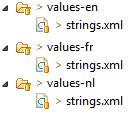
\includegraphics[scale=1]{Pictures/lang_folder.png}
	
	\subsection{Installatie}
	\label{sec:Installatie}
	De applicatie staat nog niet in de Android Play Store, maar is wel gratis te downloaden en installeren op de AMuRate website (zie sectie \ref{sec:Bronnen}: Bronnen, tools en referenties). 
	\begin{itemize}
		\item Navigeer met de Android telefoon naar de AMuRate website 
		\item Klik op `Download .apk'
		\item Navigeer naar de Downloads map en dubbel klik op `AMuRate.apk'
		\item Op het AMuRate installatiescherm klik rechtsonder op `Install'
		\item Wanneer `Application installed' tevoorschijn komt kan je klikken op `Done' om het proces te sluiten, of `Open' om de applicatie direct te starten
	\end{itemize}
	
	
	
	\newpage
	%%%%%%%%%%%%%%%
	% GUI SECTION %
	%%%%%%%%%%%%%%%
\section{Graphical User Interface}
\label{sec:GUIpics}
	Hieronder volgen enkele schermopnames van de uiteindelijke GUI met onderstaande uitleg.  \\ \newline
	\hspace*{-5pt}\makebox[\linewidth][c]{%
	\begin{tabular} {p{7cm} >{\centering\arraybackslash}p{7cm}@{\hskip 0.5in}} 
		\centering 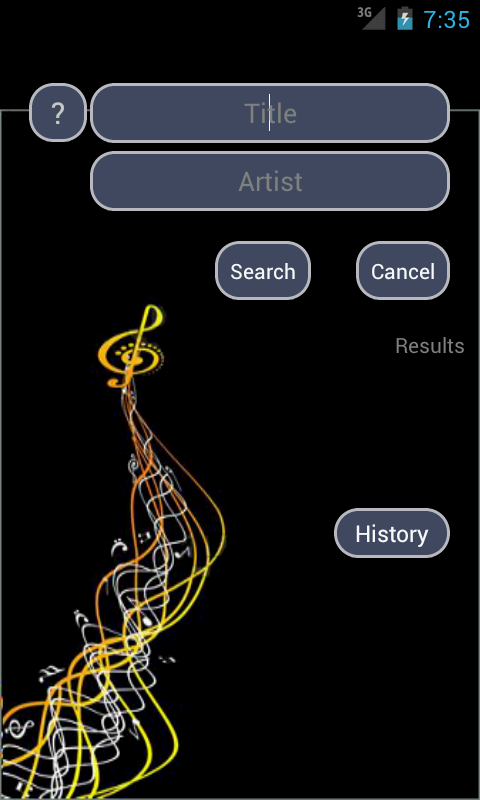
\includegraphics[scale=0.28]{Pictures/device-2013-05-25-213538.png}
		& 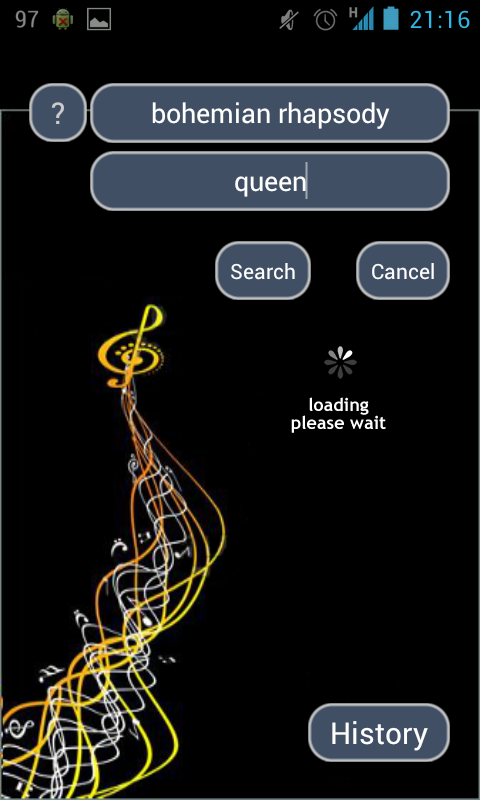
\includegraphics[scale=0.28]{Pictures/Screenshot_2013-05-24-21-16-07.png} \\
		
		\centering \figID{Start scherm.} 
		& \figID{Zoek- en downloadproces.} 
		
		\vspace{1pt} & \vspace{1pt} \\
		
	\multicolumn{1}{p{7cm}|}{%		
				Dit scherm is het start scherm en het eerste wat de gebruiker ziet wanneer de applicatie gestart wordt. Er zijn twee velden om zoektermen in te geven (een voor artiest en een voor titel). De linkerboven knop met het vraagteken erop toont de instructies van de applicatie. De submit knop start een zoekopdracht, wanneer er zoektermen opgegeven zijn. De cancel knop wist alle ingevulde gegevens. }
	&	
	\multicolumn{1}{p{7cm}} {%
		% Zoek- en downloadproces &
				In het bovenstaande scherm werden de zoektermen `Bohemian Rhapsody' en `Queen' ingevuld, en op de zoekknop geklikt. De applicatie heeft de zoektermen verwerkt en start het informatie download proces. Een spinner met `Loading...' verschijnt op het scherm om de gebruiker te laten weten dat de applicatie aan het downloaden is. } 	
				\end{tabular} 
}

%%%%%%%%%%%%%%second graphics
\hspace*{-5pt}\makebox[\linewidth][c]{%
	\begin{tabular} {p{7cm} >{\centering\arraybackslash}p{7cm}@{\hskip 0.5in}} 
		\centering 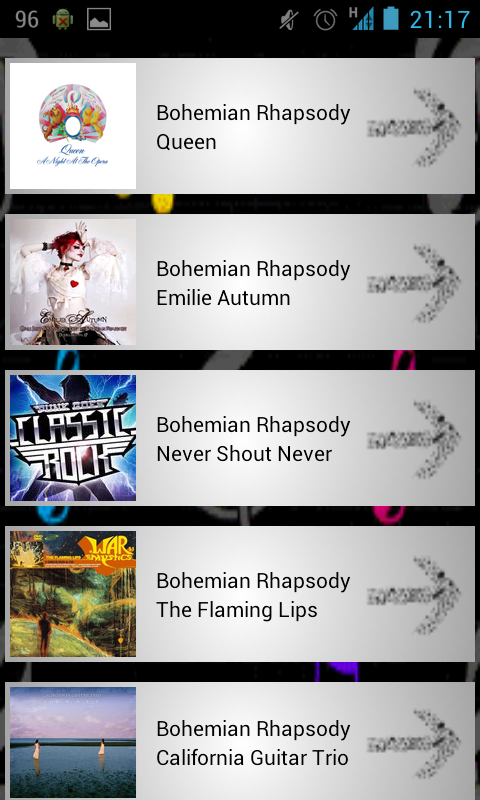
\includegraphics[scale=0.28]{Pictures/Screenshot_2013-05-24-21-17-57.png}
		& 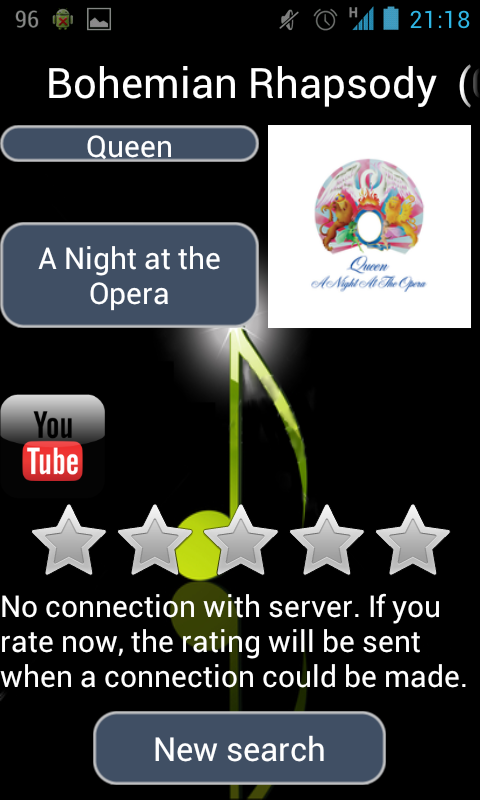
\includegraphics[scale=0.28]{Pictures/Screenshot_2013-05-24-21-18-48.png} \\
		
		\centering \figID{Lijst met alle zoekresultaten.}  
		& \figID{Gedetailleerd scherm van een lied.} 
		\vspace{1pt} & \vspace{1pt} \\
		
\multicolumn{1}{p{7cm}|}{%	% Geeft alle resultaten weer &
			De lijst die resultaten weergeeft. Men kan op elke optie klikken om naar een pagina te gaan met meer informatie. Opties die niet beschikken over een afbeelding krijgen de standaard `Niet beschikbaar' afbeelding. De anderen worden asynchroon gedownload.
 } & \multicolumn{1}{p{7cm}}{%%Weergave van een track \\	
			Dit scherm geeft de gedetailleerde pagina van een individueel lied weer. De duratie van het lied wordt getoond, het album van het lied, een afbeelding en het scoresysteem. Het gemiddelde en het aantal van alle stemmen voor dat lied wordt getoond, en 5 sterren bieden de mogelijkheid aan de gebruiker om een eigen score aan het lied toe te dienen. Helemaal onderaan bevindt zich de knop om een nieuwe zoekopdracht te starten. Wanneer men op de youtube knop klikt zal de lokale Youtube app starten. Wanneer de regel met tekst en duratie te lang wordt voor het scherm, zal de tekst als marquee bewegen.

} \\ \end{tabular}
} \newline

%%%%%%%%%%%%%%%%%%%%%%%%%%%%%%%%%%%%
%%%%%%%%%%%%%%third graphics
\hspace*{-5pt}\makebox[\linewidth][c]{%
	\begin{tabular} {p{7cm} >{\centering\arraybackslash}p{7cm}@{\hskip 0.5in}} 
		\centering 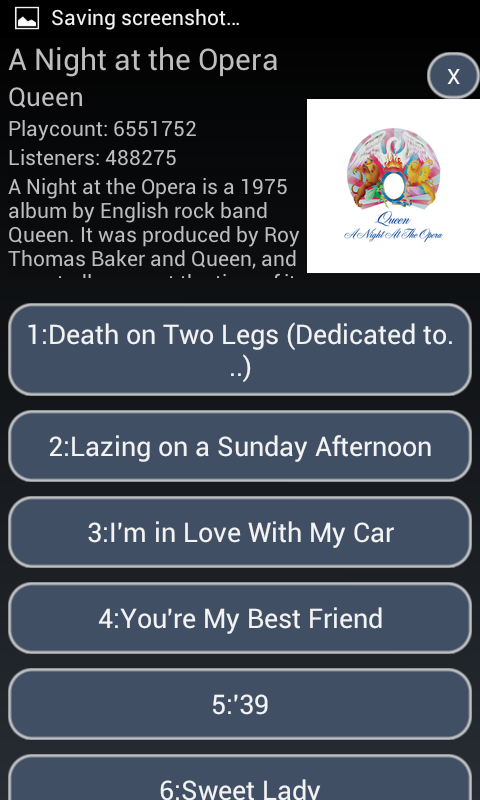
\includegraphics[scale=0.28]{Pictures/Screenshot_2013-05-24-21-20-57.png}
		& 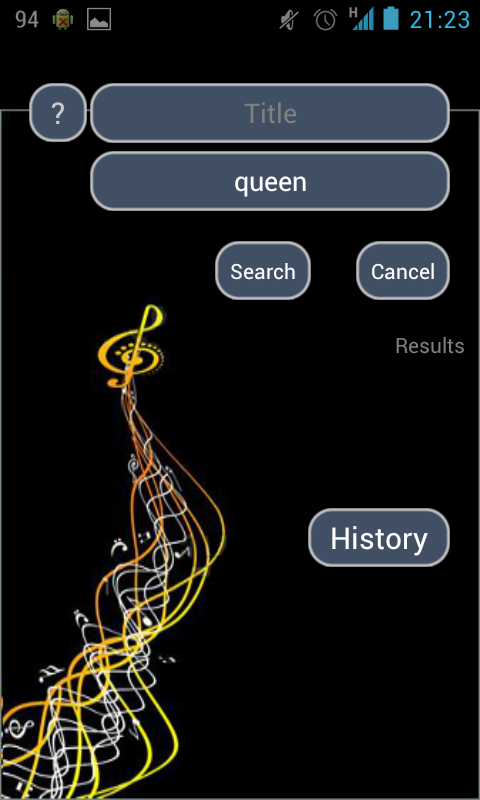
\includegraphics[scale=0.28]{Pictures/Screenshot_2013-05-24-21-23-29.png} \\
		
		\centering \figID{Gedetailleerd scherm voor een album.} 
		&  \figID{We willen hier enkel op artiestnaam zoeken.} 
		
		\vspace{1pt} & \vspace{1pt} \\
		
\multicolumn{1}{p{7cm}|}{%%Albumscherm
	Wanneer er meer album informatie beschikbaar is en de gebruiker klikt op het album, komt hij op dit scherm terecht. Het bevat informatie over een gegeven album zoals artiest, albumafbeelding, playcount, listeners, een scrollbare album informatie tekst en alle liedjes die op dat album staan. De gebruiker kan op elk lied klikken om naar de gedetailleerde liedjes pagina te gaan. 
 } & \multicolumn{1}{p{7cm}}{%
	Als we enkel het artiest veld invullen, zal er een oproep gedaan worden naar de Last.fm API om artiesten te zoeken, niet tracks. Zoals normaal verschijnt de knop `View' als er resultaten gevonden zijn, of verschijnt er een boodschap dat er geen matches waren voor de opgegeven zoekstring.
} \\ \end{tabular}
} \newline

%%%%%%%%%%%%%%%%%%%%%%%%%%%%%%%%
%%%%%%%%%%%%%%fourth graphics
\hspace*{-5pt}\makebox[\linewidth][c]{%
	\begin{tabular} {p{7cm} >{\centering\arraybackslash}p{7cm}@{\hskip 0.5in}} 
		\centering 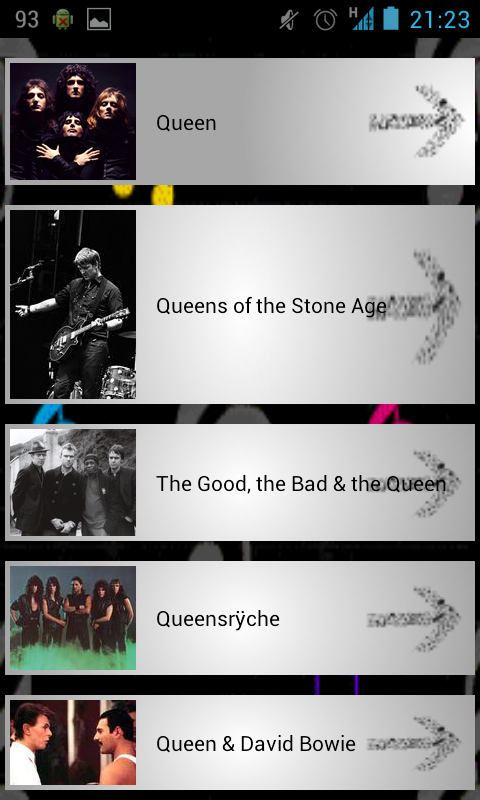
\includegraphics[scale=0.28]{Pictures/Screenshot_2013-05-24-21-23-51.png}
		& 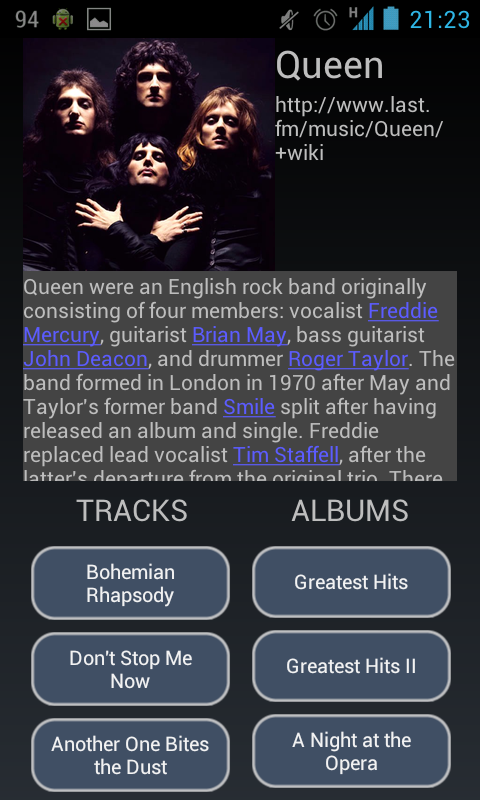
\includegraphics[scale=0.28]{Pictures/Screenshot_2013-05-24-21-23-02.png} \\
		
		\centering \figID{Gevonden artiest resultaten voor querie.} 
		&  \figID{Gedetailleerd scherm van een artiest.} 
		\vspace{1pt} & \vspace{1pt} \\
		
\multicolumn{1}{p{7cm}|}{%
 	De SearchArtistActivity is zeer gelijkaardig aan de zoek tracks pagina. We tonen een afbeelding om te helpen kiezen welke artiest de gebruiker wou bezoeken.
 } & \multicolumn{1}{p{7cm}}{%
	Wanneer een gebruiker meer informatie wilt over een artiest of groep, komt hij/zij op dit scherm terecht. Er is een link naar de wiki (als die bestaat), een scrollbare biografie, en een lijst van de artiest's top tracks en top albums. Men kan in beide lijsten scrollen en op elke item klikken om naar de gedetailleerde track/album pagina te gaan.
} \\ \end{tabular}
} \newline
%%%%%%%%%%%%%%%%%%%%%%%%%%%%%%%%%%%%
%%%%%%%%%%%%%%fifth graphics
\hspace*{-5pt}\makebox[\linewidth][c]{%
	\begin{tabular} {p{7cm} >{\centering\arraybackslash}p{7cm}@{\hskip 0.5in}} 
		\centering 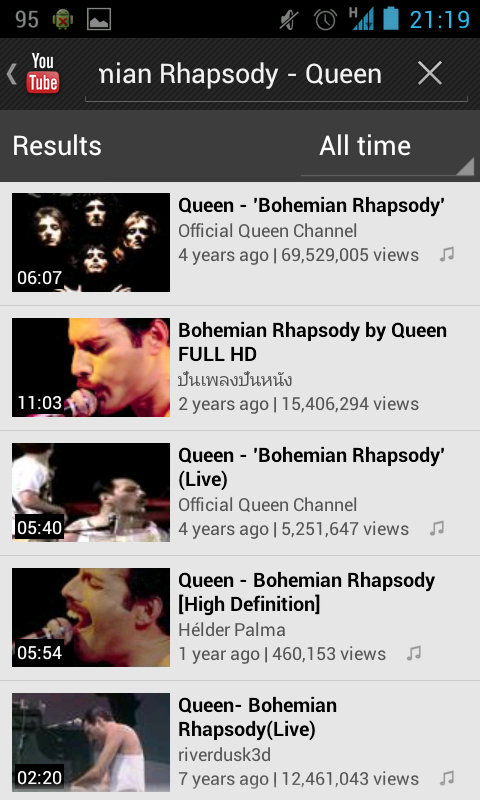
\includegraphics[scale=0.28]{Pictures/Screenshot_2013-05-24-21-19-44.png}
		& 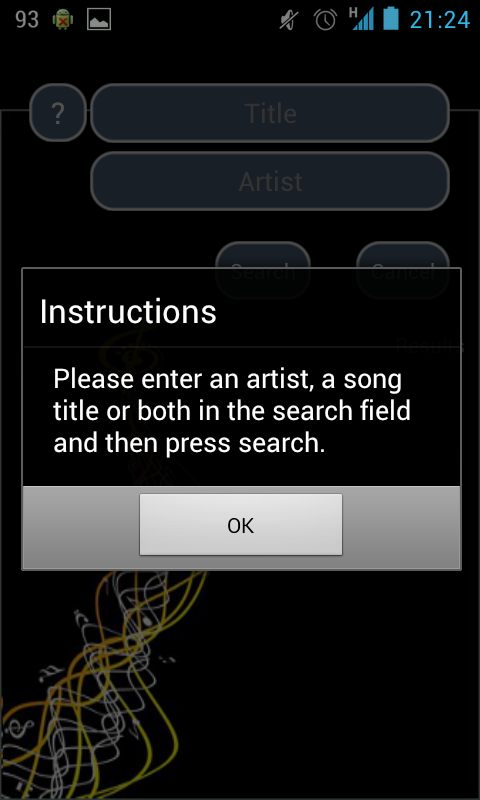
\includegraphics[scale=0.28]{Pictures/Screenshot_2013-05-24-21-24-20.png} \\
		
		\centering \figID{Link naar de youtube app.}  
		&  \figID{Instructie pop up.} 
		\vspace{1pt} & \vspace{1pt} \\
		
\multicolumn{1}{p{7cm}|}{%%
 	Wanneer iemand in de TrackActivity op de Youtube knop klikt, zal de lokale Youtube app opgeroepen worden met als zoekterm de artiest en titel van het lied, zodat de gebruiker het liedje nog eens kan afspelen voordat hij/zij een score wilt bedelen.
 } & \multicolumn{1}{p{7cm}}{%
	Als men op het vraagteken in de linksboven hoek klikt, komt deze pop-up tevoorschijn. Het geeft de instructies die nodig zijn om een eerste zoekopdracht uit te voeren.
} \\ \end{tabular}
} \newline
%%%%%%%%%%%%%%%%%%%%%%%%%%%%%%%%%%%%
%%%%%%%%%%%%%%six graphics
\hspace*{-5pt}\makebox[\linewidth][c]{%
	\begin{tabular} {p{7cm} >{\centering\arraybackslash}p{7cm}@{\hskip 0.5in}} 
		\centering 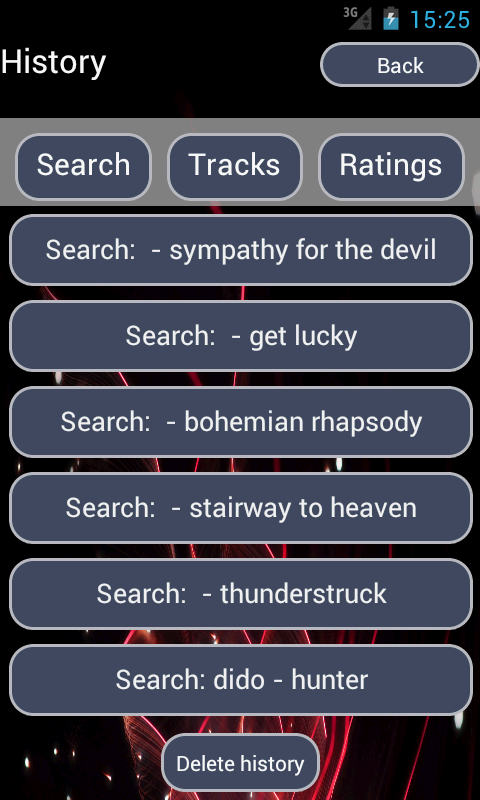
\includegraphics[scale=0.37]{Pictures/device-2013-06-02-172637track.png}
		& 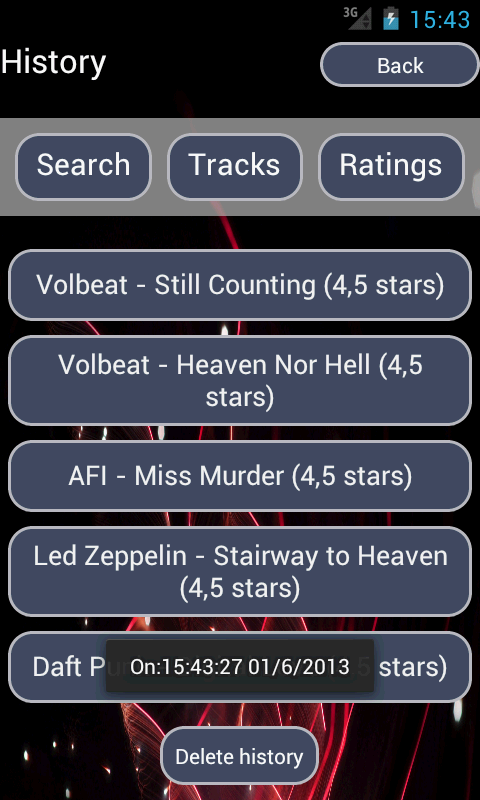
\includegraphics[scale=0.28]{Pictures/device-2013-05-31-202339000.png} \\
		
		\centering \figID{Geschiedenis scherm.}  
		&  \figID{Geschiedenis ratings.} 
		\vspace{1pt} & \vspace{1pt} \\
		
\multicolumn{1}{p{7cm}|}{%%
 	Dit is het geschiedenisscherm. Vanboven is er een knop om terug te keren naar het hoofdscherm en er vlak onder enkele tabs. De tabs zitten in een horizontale scrollbar en kunnen dus verschoven worden. Wanneer de gebruiker op een van deze tabs klikt, worden de respectievelijke geschiedenisrecords in het midden van het scherm ingeladen. Met de onderste knop kan de gebruiker deze records wissen. Op bovenstaande afbeelding zien we de `search' geschiedenis. Door op een item te klikken in de lijst, worden die zoektermen terug ingevuld in de zoekvelden van het hoofdscherm.
 } & \multicolumn{1}{p{7cm}}{%
	De `Ratings' tab geeft een overzicht van alle gegeven scores. We tonen de titel, artiest en aantal gegeven sterren. Door op een score te klikken verschijnt er een boodschap die zegt wanneer die rating precies gegeven werd.
} \\ \end{tabular}
} \newline
%%%%%%%%%%%%%%%%%%%%%%%%%%%%%%%%%%%%
%%%%%%%%%%%%%%seven graphics
\hspace*{-5pt}\makebox[\linewidth][c]{%
	\begin{tabular} {p{7cm} >{\centering\arraybackslash}p{7cm}@{\hskip 0.5in}} 
		\centering 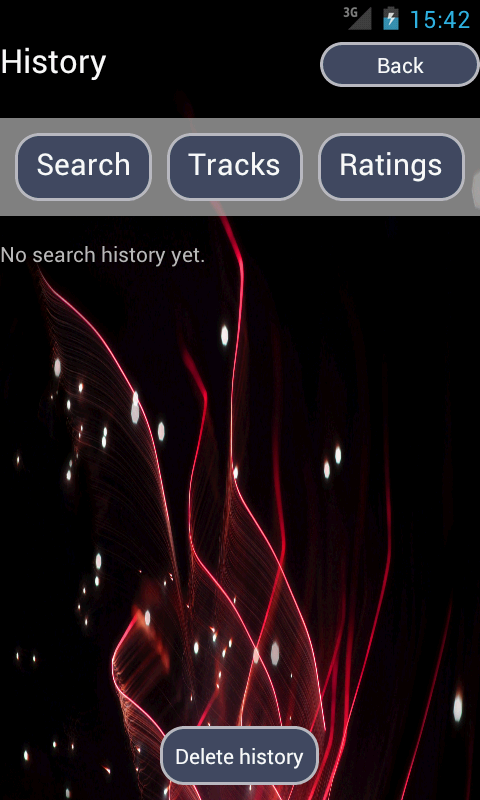
\includegraphics[scale=0.28]{Pictures/device-2013-05-31-202456.png}
		& 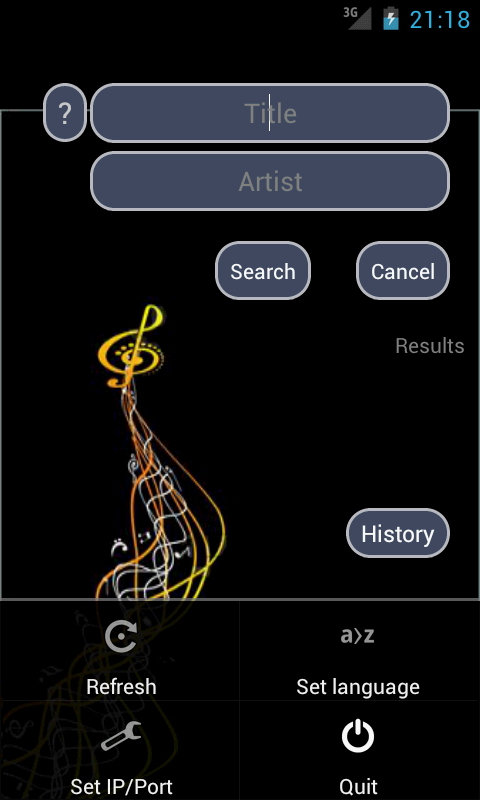
\includegraphics[scale=0.28]{Pictures/device-2013-06-01-231855menu.png} \\
		
		\centering \figID{Geschiedenis gewist.}  
		&  \figID{AMuRate menu van elk scherm.} 
		\vspace{1pt} & \vspace{1pt} \\
		
\multicolumn{1}{p{7cm}|}{%%
 	Delete history verwijdert de geschiedenis records van de huidig geopende tab.
 } & \multicolumn{1}{p{7cm}}{%
	Op bovenstaande afbeelding zien we het menu dat tevoorschijn komt wanneer de gebruiker op de `menu' knop van zijn telefoontoestel duwt. Er is een optie die het huidige scherm refresht, een optie om de taal te veranderen (zie volgende afbeelding) en een knop om de applicatie volledig af te sluiten.
} \\ \end{tabular}
} \newline
%%%%%%%%%%%%%%%%%%%%%%%%%%%%%%%%%%%%
%%%%%%%%%%%%%%eight graphics
\hspace*{-5pt}\makebox[\linewidth][c]{%
	\begin{tabular} {p{7cm} >{\centering\arraybackslash}p{7cm}@{\hskip 0.5in}} 
		\centering 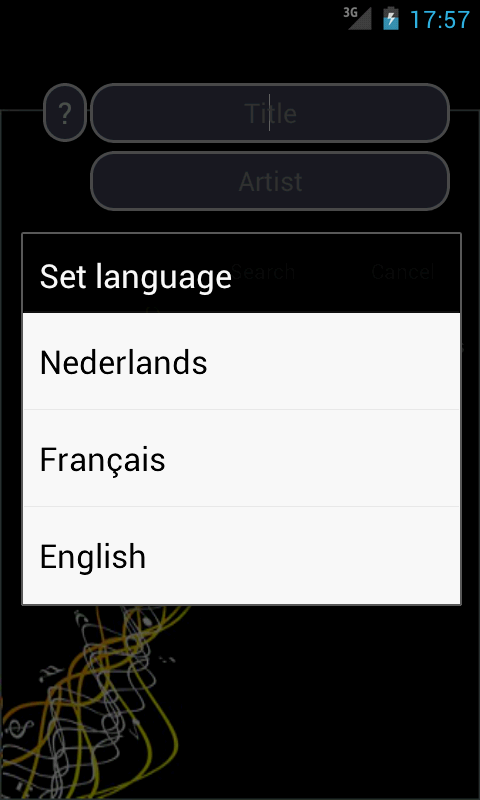
\includegraphics[scale=0.28]{Pictures/device-2013-05-31-195753.png}
		& 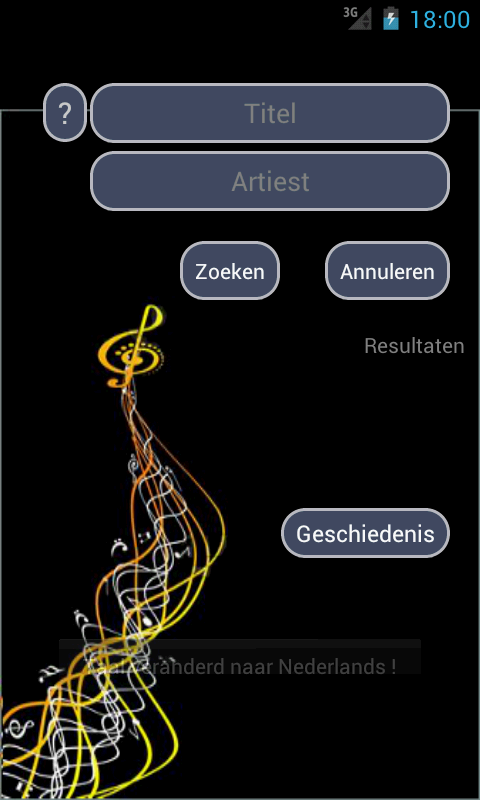
\includegraphics[scale=0.28]{Pictures/device-2013-05-31-200021.png} \\
		
		\centering \figID{Taal veranderen menu. }  
		& \figID{Taal veranderd naar Nederlands} 
		\vspace{1pt} & \vspace{1pt} \\
		
\multicolumn{1}{p{7cm}|}{%%
 	Wanneer men klikt op de menu knop om de taal te veranderen, zal hij een pop-up krijgen met de beschikbare taal-opties. Een gebruiker kan kiezen om de taal in te stellen die al actief is, dit zal niets veranderen en heeft dan dezelfde werking als een refresh. 
 } & \multicolumn{1}{p{7cm}}{%
 	Zoals we hier zien is alle tekst van de knoppen veranderd naar het Nederlands. Er kwam ook een Toast onderaan op het scherm (maar door de screenshot te nemen is die al bijna volledig vervaagd), waarop stond `Taal veranderd naar het Nederlands!'.
} \\ \end{tabular}
} \newline

%%%%%%%%%%%%%%%%%%%%%%%%%%%%%%%%%%%%
%%%%%%%%%%%%%%ninth graphics
\hspace*{-5pt}\makebox[\linewidth][c] {%
	\begin{tabular} {p{7cm} >{\centering\arraybackslash}p{7cm}@{\hskip 0.5in}} 
		\centering 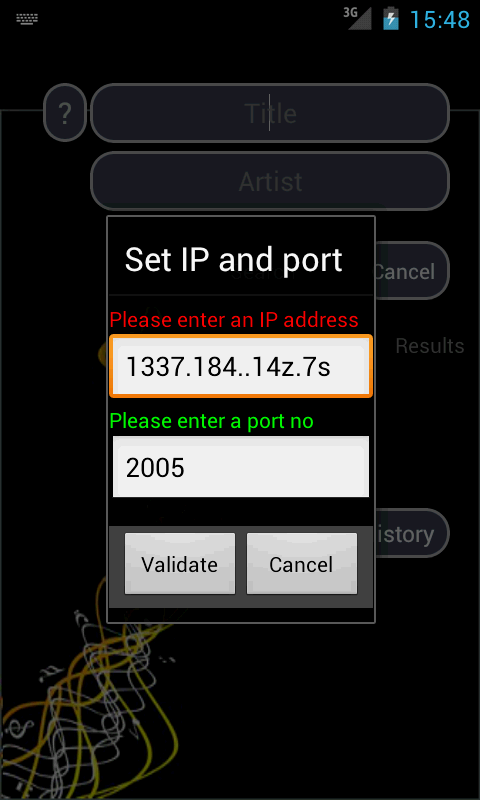
\includegraphics[scale=0.28]{Pictures/device-2013-06-01-232751iperror.png}
		& 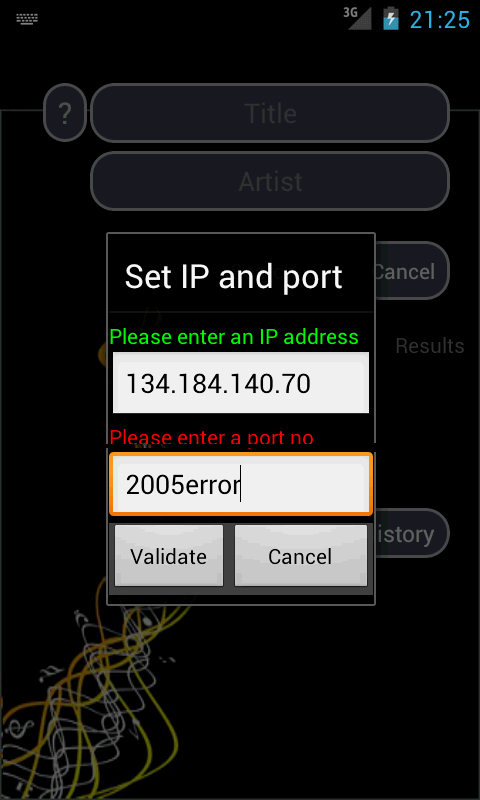
\includegraphics[scale=0.28]{Pictures/device-2013-06-01-232655porterror.png} \\
		
		\centering \figID{Validatie van IP adres faalt. }  
		& \figID{Validatie van poortnummer faalt.} 
		\vspace{1pt} & \vspace{1pt} \\
		
\multicolumn{1}{p{7cm}|}{%%
	Het gegeven IP adres wordt gevalideerd door de `InetAddressUtils' klasse. Wanneer deze validatie faalt, wordt de tekst boven dat veld in het rood gekleurd.
 } & \multicolumn{1}{p{7cm}}{%
 	Het poortnummer wordt eveneens gevalideerd wanneer de gebruiker op `Validate' klikt. Het moet eerst en vooral een nummer zijn, en moet tussen 1024 en 49151 liggen. Deze nummers komen van \href{http://www.tcpipguide.com/free/t_TCPIPApplicationAssignmentsandServerPortNumberRang-2.htm}{tcpipguide.com}. Als de validatie faalt (zoals in de afbeelding te zien is), blijft de pop-up open.  
 } \\ \end{tabular}
} \newline
%%%%%%%%%%%%%%%%%%%%%%%%%%%%%%%%%%%%
% history gui

	\newpage
%%%%%%%%%%%%%%%%%%%%%%%%%%
% Feedback %
%%%%%%%%%%%%%%%%%%%%%%%%%%
\section{Gebruiker feedback}
\label{sec:feedback}

In de laatste maand van het project werd de applicatie door een tiental vrijwilligers getest. De bedoeling was dat ze de applicatie installeren en dan enkele scores geven. Nadien konden ze via een formulier\footnote{ \url{wilma.vub.ac.be/~dsverdlo/bachproef/form307222/form.html} } uigebreid feedback geven over hun ervaring. Van de 6 inzendingen vonden alle deelnemers direct hoe ze de applicatie konden installeren, een liedje konden opzoeken en er een score aan konden geven. Gemiddeld heeft elke deelnemer 8 liedjes een score gegeven. Op één tester na gebruikten ze allemaal de Youtube knop en vonden dit een nuttige functionaliteit. Gemiddeld gaven de mensen een score van 3.5/5 op de layout. Enkele gebruikers vonden ook bugs toen ze hun telefoon omdraaiden naar landscape mode, maar die zijn nu opgelost door de applicatie niet te herladen wanneer de gsm omgedraaid wordt. 

	
%%%%%%%%%%%%%%%%%%%%%%%%%%
% Tegengekomen problemen %
%%%%%%%%%%%%%%%%%%%%%%%%%%
\section{Tegengekomen problemen}
\label{sec:Tegengekomen problemen}

	\subsection{Synchronous tasks}
	\label{sec:Synchronious tasks}
	Wanneer data binnengehaald moet worden van de API, mag die operatie niet gebeuren op de main thread van het programma, anders zal de applicatie zeer traag/onbruikbaar zijn elke keer dat er iets gedownload moet worden. Hierom werd een klasse `ServerConnect' gemaakt, die async\footnote{Asynchronous betekent dat een process tegelijkertijd naast een ander process kan werken.} data begint binnen te laden terwijl de applicatie vloeiend kan blijven voortdraaien. Door alle tijdnemende processen op een nadere
	

		
	\subsection{Veranderende MBID's}
	\label{sec:veranderendeMBID}
	In de Last.fm API hebben alle liedjes, artiesten en albums een geassociëerde MBID. Tijdens het programmeren door, viel het op dat ik scores kon geven op liedjes die normaal gezien al een score hadden gekregen van mij. Nu blijkt dat de MBID's op willekeurige tijdstippen en intervallen veranderen. In onderstaande afbeelding is een query gezien, die de verschillende MBID's weergeeft van één lied. \\
	
	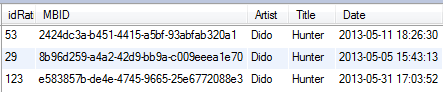
\includegraphics[scale=1]{Pictures/mbid_change.png} \\
	\figID{Verschillende MBID's voor één track.}
	
	Over deze veranderingen is geen documentatie te vinden op de Last.fm website. Het probleem van deze veranderingen is pas in mei opgemerkt, dus hier is nog geen oplossing voor ingevoerd. Een mogelijke oplossing voor dit probleem zou zijn om liedjes te identificeren via hun track en artiest. (Eventueel ook duratie.) 


%%%%%%%%%%%%%%%%%%%%%%%%
%% CONCLUSIE %%
%%%%%%%%%%%%%%%%%%%%%%%	
\newpage	
\section{Conclusie}
	\label{sec:Conclusie}
	
Toen ik aan dit bachelorproject begon, dacht ik dat het gelijkaardig zou zijn aan het vak Software Engineering, waar we in een groep van 5 mensen een mobiele transit applicatie hebben gemaakt. (Ook voor het mobiele platform Android.) In dat team zat ik wel in het team dat de server API implementeerde, en niet de Java code voor de applicatie. \\

Tijdens het uitvoeren van dit project heb ik ondervonden dat ik niet over voldoende voorkennis beschikte om alles zelf te doen. Er waren veel onverwachte elementen die opdoken, en ik heb onderzoek moeten doen over hoe men degelijke applicaties te schrijven voor Android. \\

Het was zeer leerzaam om elke stap van het project zelf voort te brengen (in tegenstelling tot de rol in het Software Engineering project). Na de eerste stappen begon de applicatie een stevigere vorm te krijgen en kon ik aan de database en de serverside beginnen. Er moest eerst research gedaan worden naar het opzetten van een server en een MySQL database, aangezien ik dit nog nooit zelf heb gedaan. \\

Een merkbare evolutie in dit project was de kwaliteit van de code. Naarmate er meer en meer onderzoek geleverd werd naar het schrijven van goede Android code, steeg de kwaliteit, leesbaarheid en becommentarisering van de broncode. \\

Door typische `problemen' tegen te komen en op te lossen, werden er veel aspecten van het coderen van een app veel duidelijker en interessante stof tot nadenken. Bijvoorbeeld mag geen enkel download-proces op dezelfde thread lopen als de gebruikers interface. Moeten er callback's\footnote{Dit is een functie die later uitgevoerd wordt, wanneer een ander proces klaar is met zijn taak.} geïmplementeerd worden, en moeten alle mogelijke acties van gebruikers in achting genomen worden. Ook de layout is belangrijk voor de eindgebruikers en hier moet voldoende tijd en aandacht in gestoken worden. \\

Dat zijn allemaal zaken die ik door dit project heb bijgeleerd. Wat ik anders gedaan zou hebben als ik terug in de tijd kon gaan, is meer commentaar zetten bij mijn code, en vanaf het begin oog houden op uitbreidbaarheid. (Dit heeft me naar het einde van het project veel tijd gekost.) \\

Wat er in de toekomst nog aan de app bijgemaakt kan worden, is een integratie met andere media applicaties (zoals Shazam, TrackID, MusicPlayer, ...) om gebruikers sneller hun favoriete liedjes op te laten zoeken en te raten. Verder ook de muziek recommendering, die op basis van gegeven scores, nieuwe muziek kan voorstellen aan de gebruikers. \\

Ik durf wel te zeggen dat ik zelf zeer tevreden ben met de eind applicatie, met het werk dat ik heb geleverd, en de ervaring die ik heb opgedaan. Mobiele apps zijn zeker aanwezig in de toekomst en ik zou er later meer mee willen werken.

%%%%%%%%%%%%%%%%%%%%%%%%
%% BRONNEN %%
%%%%%%%%%%%%%%%%%%%%%%%	
\newpage	
\section{Bronnen, tools en referenties}
	\label{sec:Bronnen}

	\begin{itemize}
		
	\item \textbf{Eclipse} \\
	Programmeerplatform Eclipse (Juno) werd gebruikt voor de implementatie en emulatie.	\\
	\url{http://www.eclipse.org/}

	\item \textbf{Android Development Toolkit (ADT)} \\
	Deze plug-in bevat alle benodigdheden om programma's voor Android in Eclipse te bouwen en testen.\\
	\url{http://developer.android.com/sdk/index.html}
	
	\item \textbf{MySQL} \\
	Op MySQL workbench werd de data collection aangemaakt en kon de luisterende socket aangemaakt worden. \\
	\url{http://www.mysql.com/}	
	
	\item \textbf{LucidChart} \\
	Op deze website werden de diagrammen en andere afbeeldingen in dit document gegenereerd.\\
	\url{lucidchart.com}
	
	\item \textbf{AMuRate homepagina} \\
		\url{http://dsverdlo.github.com/AMuRate}
		
	\item \textbf{Android} \\
		\url{http://www.android.com/}
		
	\item \textbf{Ice Cream Sandwich} \\
		\url{http://www.android.com/about/ice-cream-sandwich/}	
		
	\item \textbf{Last.fm} \\
		\url{http://www.last.fm/home}	
		
	\item \textbf{Github} \\
		\url{https://github.com/}



	\end{itemize}



\end{document}
